\documentclass[a4paper,12pt]{article}
\usepackage{graphicx}
\begin{document}
\pagenumbering{roman} 
\tableofcontents
 \newpage
 \pagenumbering{arabic}
\newpage
\section{INTRODUCTION}\vspace{5mm}
\subsection{Project Profile}\vspace{5mm}
VIVID app is a customized mobile application that can help you in various ways. The main language of programming will be android. Its main  aim is simplifying and improve the selling process for the owner. Minimize manual data entry and ensure data accurancy and security. Customer will able to view product menus and their price, according to their interest. Admin can view the details of selling buying, stock, report generation.
\par  \vspace{2mm}  
Usage of mobile phones has increased in the past year. India stands second in the world, in the number of active mobile phones. Today, out of the 6 billion mobile phones in the world, close to 1 billion is being used in India. This comes to about 70 percentage  of our current population. Every month sees an increase of around 6 million subscribers. That, in fact, is a lot of numbers.
With the increase in the number and make of mobile phones, there comes a demand for better applications.
\par  \vspace{2mm}  
The new system entitled VIVID Application provides a lot of services to the user as compared to the existing system. It provides a better way for the users to get all the information needed as quick as possible from anywhere in the world. The user can get the information regarding different available service details.Consultants offer advice and expertise to organisations to help them improve their business performance in terms of operations, profitability, management, structure and strategy. ... The work stretches across a variety of areas, including management, strategy, IT, finance, marketing,.
\subsection{Organisation Overview}\vspace{5mm}
             Entrepreneurs such as you are increasingly discovering the need for an excellent website that gather a wide audience. Our job is to create this platform for you- a simple yet creative website to bring together your target demographic. Our services include creative and efficient quality web designing, web development, SEO services, Website maintenance, mobile applications and so forth. Essentially, we are the solution for all your web portal needs.
\newpage
\par  \vspace{2mm} 
            We pride in our analyzing and researching skills that helps us provide you with an easy-to-use, professional website that appeals to both your current and prospective clientele. We are committed to providing the best services in web technology with a vision of satisfied and contend clients. Let us take your business to the web so that millions of people across the world can access it. Allow us to help reach your goal faster.
\par  \vspace{2mm} 
Cazablaze Technologies PVT Lmtd is a major international force in IT consulting and services. Utilizing our broad range of Web-based solutions, we address and resolve the integration  and solutions needs of today's IT users for both hardware and software. Our integrated quality information system helps us manage all aspects of high quality software production in our organization. Internal quality assessments are done twice a year with the intention of identifying quality issues and areas of improvement. The assessment focuses on customer rating on product quality, our service levels as well as the effectiveness of the quality system.
\par  \vspace{2mm} 
Cazablaze expert creative services team delivers the following services:  
 \begin{enumerate}
\item Branding
\item Web Application
\item Consultancy
\item SEO
\item Software Development
\item Web Designing
\item SMO
\item Digital Marketing
\item Mobile App Development
\item Custom ERP Solutions
\item Consulting Services
\end{enumerate}          

\vspace{2mm}
\newpage
\subsection{Overview of The System}\vspace{5mm}
Android offers a unified approach to application development for mobile devices which means developers need only develop for Android, and their applications should be able to run on different devices powered by Android.Consultants offer advice and expertise to organisations to help them improve their business performance in terms of operations, profitability, management, structure and strategy. The work stretches across a variety of areas, including management, strategy, IT, finance, marketing. This new application introduced with a vision of bringing the important services in our fingerprints.
 \par  \vspace{2mm}              
 \begin{enumerate}
\item Mobile  application  ( android and IOS application)
\item Web portal
\end{enumerate}
\subsection{Scope of The Project}\vspace{5mm}
“Mobile is the future of Software Development” – Google’s Eric Schmidt.
Usage of mobile phones has increased in the past year. India stands second in the world, in the number of active mobile phones. Today, out of the 6 billion mobile phones in the world, close to 1 billion is being used in India. This comes to about 70 percentage  of our current population.
 \par  \vspace{2mm}  
 Every month sees an increase of around 6 million subscribers. That, in fact, is a lot of numbers.
With the increase in the number and make of mobile phones, there comes a demand for better applications. And in turn, huge scope of android mobile application development in India. Now, this puts a light on why companies like Nokia, BlackBerry, Samsung, HTC, Motorola, Google and many others are going wild with their innovations – increase in the need and use of Mobile Applications.
  \par  \vspace{2mm}  
Android is an open-source Linux-based operating system designed mainly for smart phones and tablets. It is maintained as an open source project by Google. This open source code and licensing allows the developers and device manufacturers to modify the software according to their needs. Android platform has brought about cutting-edge technologies in app development.Owing to the popularity of Android, Mobile Apps development industries are considering Android Application Development as one of the best remunerative business opportunities.
 \par  \vspace{2mm}   The need to hire knowledgeable mobile application developer is intense.India is considered as a country with several globally recognized IT hubs.One of the main reasons for this is that software as a service is highly cost effective.
 \par  \vspace{2mm}
 Before the acceptance of Android, the mobile app development industry was dominated by Proprietary OS like Symbian and iOS. With Android, came the option for dynamic app development at a lower cost. When thinking of the scope of Android Application Development in India, we can take these three primary notions into consideration:
\begin{itemize}
\item Revenue : The need for inventive App Developers are increasing in the current job market. Mobile application development can also be taken up as a part time job, where you can create your own applications and submit it to the Google Play store which can be downloaded. Google adsense ads can be displayed in your application which again provides monetary gains.
\item Ease of use : Learning Android Programming is fairly easy and app development is cost effective. Any software developer who can think out of the box will be able to put Android into extraordinary use.
\item Support :The most important attraction of Android is backing by Google.
\end{itemize}
\par\vspace{2mm}
\newpage
\section{ABOUT THE DEVELOPING TOOLS}\vspace{5mm}
\subsection{Introduction to PHP}\vspace{2mm}
PHP is a server-side scripting language designed for web development but also used as a general-purpose programming language.  While PHP originally stood for Personal Home Page, it now stands for PHP: Hypertext Pre-processor, PHP code can be simply mixed with HTML code, or it can be used in combination with various templating engines and web frameworks. PHP code is usually processed by a PHP interpreter, which is usually implemented as a web server's native module or a Common Gateway Interface (CGI) executable. After the PHP code is interpreted and executed, the web server sends resulting output to its client, usually in form of a part of the generated webpage; for example, PHP code can generate a web page's HTML code, an image, or some other data. PHP has also evolved to include a command-line interface (CLI) capability and can be used in standalone graphical applications.\par\vspace{2mm}
The canonical PHP interpreter, powered by the Zend Engine, is free software released under the PHP License. PHP has been widely ported and can be deployed on most web servers on almost every operating system and platform, free of charge. Despite its popularity, no written specification or standard existed for the PHP language until2014, leaving the canonical PHP interpreter as adefacto standard. Since 2014, there is ongoing work on creating a formal PHP specification.\par\vspace{2mm}
There are two primary ways for adding support for PHP to a web server as a native web server module, or as a CGI executable. PHP has a direct module interface called Server Application Programming Interface (SAPI), which is supported by many web servers including Apache HTTP Server, Microsoft IIS, Netscape (now defunct) and iPackage set. Some other web servers, such as Omni HTTPd, support the Internet Server Application Programming Interface (ISAPI), which is a Microsoft's web server module interface.
\par
Usage:-\par\vspace{2mm}
PHP is a general-purpose scripting language that is especially suited to server-side web development, in which case PHP generally runson a web server. Any PHP code in a requested file is executed by the PHP runtime, usually to create dynamic web page content or dynamic images used on websites or elsewhere .It can also be used for command-line scripting and client-side graphical user interface (GUI)applications.. PHP can be deployed on most web servers, many operating systems and platforms , and can be used with many relational database management systems (RDBMS). Most web hosting providers support PHP for use by their clients. It is available free of charge, and the PHP Group provides the complete source code for users to build, customize and extend for their own use. 
The LAMP architecture has become popular in the web industry as a way of deploying web applications.PHP is commonly used as the P in this bundle alongside Linux , Apache and MySQL , although the P may also refer to Python , Perl , or some mix of the three. Similar packages, WAMP and MAMP, are also available for Windows and OS X , with the first letter standing for the respective operating system. 
\par\vspace{2mm}
   \subsection{My SQL}\vspace{5mm}
Structured Query Language (SQL), in computer science, a database sub language used in querying, updating and managing relational databases. Derived from an IBM research project that created Structured English Query Language (SEQUEL) in the 1970’s SQL is accepted standard in database products. Although it is not a programming language in the same sense as C or PASCAL, SQL can either be used in formulating interactive queries or be embedded in as application as for handling data.Microsoft SQL server is a relational database that runs on the Windows NT operating system. SQL (RDBMS) is a widely accepted industry standard for defining , changing and managing data and controlling how changes to the database are made by using tables, index keys rows and columns to store data.\par\vspace{2mm}
Microsoft SQL server is a relational database that runs on the Windows NT operating system. SQL (RDBMS) is a widely accepted industry standard for defining , changing and managing data and controlling how changes to the database are made by using tables, index keys rows and columns to store data. 
\par\vspace{2mm}
The MySQL software delivers a very fast, multi-threaded, multi-user, and robust SQL (Structured Query Language) database server. MySQL Server is intended for mission-critical, heavy-load production systems as well as for embedding into mass-deployed software. Oracle is a registered trademark of Oracle Corporation and/or its affiliates. is a trademark of Oracle Corporation and/or its affiliates, and shall not be used by Customer without Oracle's express written authorization. Other names may be trademarks of their respective owners. 
The MySQL software is Dual Licensed. Users can choose to use the MySQL software as an Open Source product under the terms of the GNU General Public License. 
\subsection{Android}\vspace{5mm}
Android is a mobile operating system developed by Google, based on the Linux kernel  and designed primarily for touch screen mobile devices such  as smart phones and tablets. Android's user interface is mainly based on direct manipulation, using touch gestures that loosely correspond to real-world actions, such as swiping, tapping and pinching, to manipulate on-screen objects, along with a virtual keyboard for text input.. In addition, Google has further developed Android TV for televisions, Android Auto for cars, and Wear OS for wrist watches, each with a specialized user interface. Variants of Android are also used on game consoles, digital cameras, PCs and other electronics.\par\vspace{2mm}
Android's source code is released by Google under an open source license, although most Android devices ultimately ship with a combination of free and open source and proprietary software, including proprietary software required for accessing Google services. Android is popular with technology companies that require a ready-made, low-cost and customizable operating system for high-tech devices.
\par\vspace{2mm}
 Its open nature has encouraged a large community of developers and enthusiasts to use the open-source code as a foundation for community-driven projects, which deliver updates to older devices, add new features for advanced users or bring Android to devices originally shipped with other operating systems.Initially developed by Android Inc., which Google bought in 2005, Android was unveiled in 2007, with the first commercial Android device launched in September 2008. The operating system has since gone through multiple major releases, with the current version being 8.1 "Oreo", released in December 2017. The core Android source code is known as Android Open Source Project (AOSP), and is primarily licensed under the Apache License.\par\vspace{2mm}
Android is also associated with a suite of proprietary software developed by Google, including core apps for services such as Gmail and Google Search, as well as the application store and digital distribution platform Google Play, and associated development platform. These apps are licensed by manufacturers of Android devices certified under standards imposed by Google such as Amazon.com's Fire OS, which utilize its own equivalents to these Google Mobile Services.
\par\vspace{2mm}
\newpage
\subsection{Netbeans}\vspace{5mm}
Netbeans is an integrated development environment (IDE) for developing primarily with Java, but also with other languages, in particular PHP, C/C++, and HTML5.It is also an application platform framework for Java desktop applications and others. The NetBeans IDE is written in Java and can run on Windows, OS X, Linux, Solaris and other platforms supporting a compatible JVM. \par\vspace{2mm}
The Net Beans Platform allows applications to be developed from a set of modular software components called modules. Applications based on the Net Beans Platform (including the Net Beans IDE itself) can be extended by third party developers. Framework for simplifying the development of JavaSwing desktop applications.
\par\vspace{2mm}
 The Net Beans IDE bundle for Java SE contains what is needed to start developing Net Beans plugging and Net Beans Platform based applications; no additional SDK is required. Applications can install modules dynamically. Any application can include the Update Centre module to allow users of the application to download digitally signed upgrades and new features directly into the running application.
\par\vspace{2mm}
 Reinstalling an upgrade or a new release does not force users to download the entire application again. The platform offers reusable services common to desktop applications, allowing developers to focus on the logic specific to their application. 
\par\vspace{2mm}The JAVA community is provided a few option including NetBeans and the long time font runner the eclipse IDE.The Eclipse has lost some of its market share over the years to Intel.
Neither Eclipse or not Beans is just an IDE.They are entire platform NetBeans describe itself as an IDE that lets you quickly and easily develop java desktop, mobile and web application as well as HTML5 application with HTML.\par\vspace{2mm}

It’s a great tool for large scale projects and makes it easier to bring on new developer because its structure is visible.NetBeans is module driven-everything in NetBeans happen via modules, which power and extends all its functionalities. They are reusable.
It is excellent for converting to JAVA8. 
\par\vspace{2mm}
\subsection{Wordpress}\vspace{5mm}
WordPress is an open source Content Management System (CMS), which allows the users to build dynamic websites and blogs. WordPress is the most popular blogging system on the web and allows updating, customizing and managing the website from its back-end CMS and components. 
WordPress is an Content Management System (CMS), which is open source and was created to manage blogs. WordPress allows you to easily create and manage your blogs and websites content without coding and it can be used to create fully operational website. 
\par\vspace{2mm}
The Content Management System (CMS) is a software which stores all the data such as text, photos, music, documents, etc. and is made available on your website. It helps in editing, publishing and modifying the content of the website.
\par\vspace{2mm}
Management System (CMS) is a application software that provides you an easy environment to manage your digital content data such as text, images, music, documents etc. 
WordPress was initially released on 27th May, 2003 by Matt Mullenweg and Mike Little. WordPress was announced as open source in October 2009. 
\par\vspace{2mm}

\subsection{GIT}\vspace{2mm}
Git  is a version control system for tracking changes in computer files and coordinating work on those files among multiple people. It is primarily used for source code management in software development,but it can be used to keep track of changes in any set of files. As a distributed revision control system it is aimed at speed, data integrity,and support for distributed, non-linear workflows.Git was created by Linus Torvalds in 2005 for development of the Linux kernel, with other kernel developers contributing to its initial development.[12] Its current maintainer since 2005 is Junio Hamano.As with most other distributed version control systems, and unlike most client–server systems, every Git directory on every computer is a full-fledged repository with complete history and full version tracking abilities, independent of network access or a central server.Git is free software distributed under the terms of the GNU General Public License version 2.
\newpage
\subsubsection{Characteristics}\vspace{2mm}
Git's design is a synthesis of Torvalds's experience with Linux in maintaining a large distributed development project, along with his intimate knowledge of file system performance gained from the same project and the urgent need to produce a working system in short order. These influences led to the following implementation choices;
\begin{enumerate}
\item Strong support for non-linear development
\item Distributed development
\item Compatibility with extant systems and protocols
\item  Efficient handling of large projects
\item Cryptographic authentication of history
\item Garbage accumulates until collected
\item Periodic explicit object packing
\end{enumerate}\par
Another property of Git is that it snapshots directory trees of files. The earliest systems for tracking versions of source code, Source Code Control System (SCCS) and Revision Control System (RCS), worked on individual files and emphasized the space savings to be gained from interleaved deltas (SCCS) or delta encoding (RCS) the (mostly similar) versions. Later revision control systems maintained this notion of a file having an identity across multiple revisions of a project. However, Torvalds rejected this concept.Consequently, Git does not explicitly record file revision relationships at any level below the source code tree.Git implements several merging strategies; a non-default can be selected at merge time:
\begin{enumerate}
\item { resolve:} the traditional three-way merge algorithm.
\item {recursive:} This is the default when pulling or merging one branch, and is a variant of the three-way merge algorithm.
\item {octopus:} This is the default when merging more than two heads.
\end{enumerate}\par\vspace{2mm}
\subsubsection{Implementations}\vspace{2mm}
Git is primarily developed on Linux, although it also supports most major operating systems including BSD, Solaris, macOS, and Windows.The first Microsoft Windows port of Git was primarily a Linux emulation framework that hosts the Linux version. Installing Git under Windows creates a similarly named Program Files directory containing the MinGW port of the GNU Compiler Collection, Perl 5, msys2.0 (itself a fork of Cygwin, a Unix-like emulation environment for Windows) and various other Windows ports or emulations of Linux utilities and libraries.
\par\vspace{2mm} Currently native Windows builds of Git are distributed as 32 and 64-bit installer.The JGit implementation of Git is a pure Java software library, designed to be embedded in any Java application. JGit is used in the Gerrit code review tool and in EGit, a Git client for the Eclipse IDE.The Dulwich implementation of Git is a pure Python software component for Python 2.7, 3.4 and 3.5.The libgit2 implementation of Git is an ANSI C software library with no other dependencies, which can be built on multiple platforms including Windows, Linux, macOS, and BSD.
\par\vspace{2mm}It has bindings for many programming languages, including Ruby, Python, and Haskell.JS-Git is a JavaScript implementation of a subset of Git.\vspace{2mm}

\subsubsection{GIT Server}\vspace{2mm}
As Git is a distributed version control system, it can be used as a server out of the box. Dedicated Git server software helps, amongst other features, to add access control, display the contents of a Git repository via the web, and help managing multiple repositories. Remote file store and shell access: A Git repository can be cloned to a shared file system, and accessed by other persons. It can also be accessed via remote shell just by having the Git software installed and allowing a user to log in.
\newpage
\subsubsection{Security}\vspace{2mm}
Git does not provide access control mechanisms, but was designed for operation with other tools that specialize in access control.An attacker could perform arbitrary code execution on a target computer with Git installed by creating a malicious Git tree (directory) named .git (a directory in Git repositories that stores all the data of the repository) in a different case (such as .GIT or .Git, needed because Git doesn't allow the all-lowercase version of .git to be created manually) with malicious files in the .git/hooks subdirectory (a folder with executable files that Git runs) on a repository that the attacker made or on a repository that the attacker can modify.
\par\vspace{2mm}
 If a Windows or Mac user pulls (downloads) a version of the repository with the malicious directory, then switches to that directory, the .git directory will be overwritten (due to the case-insensitive trait of the Windows and Mac filesystems) and the malicious executable files in .git/hooks may be run, which results in the attacker's commands being executed. An attacker could also modify the .git/config configuration file, which allows the attacker to create malicious Git aliases (aliases for Git commands or external commands) or modify extant aliases to execute malicious commands when run. The vulnerability was patched in version 2.2.1 of Git, released on 17 December 2014, and announced on the next day.
\par\vspace{2mm}
\newpage
\section{SYSTEM ANALYSIS}\vspace{5mm}
\subsection{Introduction}\vspace{5mm}
System Analysis works with users to identify goals and build system to achieve them. System Analysis is an important phase of any system development process.  System analysis is a step-by-step process used to identify and develop or acquire the software need to control the processing of specific application. System analysis is a continuing activity the stages of the systems development. The system is studied to the minute’s details and analyzed. In analysis, a detailed study of these operation performed by a system and their relationships within and outside of the system is done.System analysis is a general term that refers to an orderly, structured process for identifying and solving problems. We call system analysis process life cycle methodology, since it relates to four significant phases .They are:\vspace{2mm}
\begin{enumerate}
\item Study phase
\item Design phase
\item Development phase
\item Implementation phase
\end{enumerate}
\par\vspace{2mm}
Analysis implies the process of breaking something into parts so that the whole maybe understood. The definition of system analysis includes not only the process of analysis but also that of synthesis, which implies the process of putting together to form a new one. All activities associated with each life cycle phase must be performance, management,documentation of the activities related to the life cycle phases of a computer based business system. In the study phase a detailed study of the project is made and clear picture of the project should be in mind by this time. In the design phasethe designing of the input, output and table designs are made. In the development phase is where the physical designing of the  input- output screens and coding of the system is done. In the system implementation actually implements the system by making necessary testing.
\subsection{Existing System}\vspace{5mm}
The existing systems has lot of drawbacks.Thus making it time consuming. It is error prone as users may give false information which is not approved by the admin.Admin register the information of employees. If any modifications or updates are required in the profile of any user, it has to be done manually. This is tedious and time consuming, lack of security of data, took more man power, consumes large volume of paper and space. This process is so difficult when number of employees and flower increases. 
\subsubsection{Limitations of Existing System}
\begin{enumerate}
\item Time Consuming.
\item Lack of efficiency.
\item Error Prone.
\item Lack of security.
\item Not informative.
\item Involves a lot of human efforts.
\item Cannot Upload and Download the latest updates.
\item No use of Web Services and Removing.
\item Risk of mismanagement 
\item Accuracy is less.
\item The system lacks integrity and security.
\item Highly time consuming.
\item Data redundancy and inconsistency.
\item Involves a lot of human efforts.

\end{enumerate}
\subsection{Proposed System}\vspace{5mm}
The new system entitled VIVID Application provides a lot of services to the user as compared to the existing system. It provides a better way for the users to get all the information needed as quick as possible from anywhere in the world. The user can get the information regarding different available service details.Its main  aim is simplifying and improve the selling process for the owner. Minimize manual data entry and ensure data accurancy and security.Customer will able to view product menus and their price, according to their interest. Admin can view the details of selling buying, stock, report generation. This system provides the most up-to-date services.
\subsubsection{ Advantages}
\vspace{5mm}
The system is very simple in design and to implement. It has got following features.
\begin{enumerate}
\item High speed
\item Transparency
\item Time saving
\item System dependent
\item Error free
\item Provide service to anyone at any time.
\item Efficient
\item Informative
\item Secure
\end{enumerate}
\newpage
\subsubsection{Menu Level Description}
 The different modules that will make the whole system are as follows.The project contains 2 modules and each containe 5 forms:\vspace{2mm}
\begin{enumerate}
\item{Admin Login }\par\vspace{2mm}
The Admin can login with their user name and password. They can view flower details, Stock details and employee Details.
\item{Flower Registration }\par\vspace{2mm}
Admin  can add, delete, edit the flower details.

\item{Salesman Registration }\par\vspace{2mm}
Admin  can add, delete, edit the Salesman details.

\item{Stock }\par\vspace{2mm}
 Stock Section contain the stock details of the shop if a salesman search the stock details when the customer orders flower more than the stock. It displays the order is out of the stock to the salesman.

\item{Report Generation }\par\vspace{2mm}
It will displayed the total amount of flowers including if their any decoration fee, and their will be a facility to make a printed Report.

\end{enumerate}
\newpage
\subsection{Feasibility Study}\vspace{5mm}
             The prime objective of feasibility study is to ensure that the problem is worth to be solved. At this stage a cost benefit analysis is performed to assertion that the benefit from the system will over rule the cost associated with the whole analysis, design and development of the new system. An important outcome of the preliminary investigation determining whether the system required is feasible.\par\vspace{2mm}
 Feasibility study is a test of proposed system regarding its efficiency, impact on the organization, ability to meet the needs of users and effective use of resources. Thus, when a new project is proposed, it normally goes through a feasibility study before it is approved for development.\par\vspace{2mm}
            All the projects are given unlimited resources and infinite time. Unfortunately, the development process of a computer based system is time bound and feasibility and risk analysis are related in many ways. If project risk is great, the feasibility of producing the quality software is reduced. \par\vspace{2mm}
There are three aspects in the feasibility study portion of the preliminary investigation.
\begin{enumerate}
\item Technical Feasibility 
\item Economic Feasibility
\item Behavioural Feasibility
\end{enumerate}\vspace{2mm}
\newpage

\subsubsection{Technical Feasibility}\vspace{2mm}
               It is a study of function, performance and constraints that may affect the ability to achieve acceptable system. The technical requirements for the ‘VIVID’ are currently available and are widely used. The technology used is found to be optimal for the system and are able to withstand the complexities, which are inherent to the system.The assessment of technical feasibility must be based on an outline design of the system requirements in terms of input, output, files, programs and procedures.
\par\vspace{2mm}
 This study checks the technical aspects of system. Minimum requirements of the proposed system are a computer and internet connectivity, which will not add any additional expense in implementing the system. This software is simple to use and manage.Online Freelancer system also uses the minimum technologies for the creation of the web based application. 
\par\vspace{2mm}
The technology used is found to be optimal for the system and are able to withstand the complexities, which are inherent to the system.The assessment of technical feasibility must be based on an outline design of the system requirements in terms of input, output, files, programs and procedures. The existing system has also required minimum technical requirements. So the proposed system is said to be technically feasible.
\par\vspace{2mm} The main points that are considered to prove that the project is technically feasible are:
\begin{enumerate}
\item The present technology is sufficient to develop the project.
\item The proposed system provides adequate response to the user.
\item The system can be expanded and developed.
\item The project outputs given are reliable and it is easy to access.
\end{enumerate}
\newpage
\subsubsection{Economic Feasibility}\vspace{2mm}
Economic feasibility is a method for evaluating the effectiveness of a candidate system. This study is mainly concerned with cost-benefit analysis that is how much money the user is investing in any system and how much he is getting as a benefit in output. Our project is Economical Feasible because anyone uses this software would need only to buy the machine. Our hardware requirement is not too expensive. The money and human effort needed for the existing system is high .In the new system benefits outweigh costs. So as compare to cost the project is economically feasible.
We conduct an economic feasibility study for this system and it also uses minimum hardware requirements that are already used in the existing system .In existing system manual records are used for storing details. The system is cost effective because of its compatibility and effort saving nature. The cost benefit ratio is very small and hence the proposed system is feasible.
\par\vspace{2mm}
Here an evaluation of development cost weighted against the ultimate income or benefit derived from the developed system. The cost for the development of the project has been evaluated and we want to check that the cost does not exceed beneficial cost of the system. Economic and Financial analysis is used for evaluating the effectiveness of the candidate system.\par
This project also under gone economic feasibility study and found that it is feasible. Because php is a free open source software and generally runs on a web server. So the cost for development does not exceed its beneficial cost.
\subsubsection{Behavioural Feasibility}\vspace{2mm}
This is also known as operational feasibility.The new system is very much easier and user friendly than the existing system. It satisfies the requirements identified in the requirements analysis phase of system development. It reduces the operational time considerably. Operational cost is very less. The maintenance and modification of the new system needs very less human effort. Using command buttons throughout the application programs enhances the operational feasibility. 
\par\vspace{2mm}The new system is operationally feasible and makes the operations simpler and quite easier. Operational feasibility is dependent on human resources available for the project and involves projecting whether the system will be used if it is developed and implemented. One of the main problems faced during the development of the new system is getting the acceptance from the user. People are inherently resistant to change and so estimate should be made of how strong a reaction the user is likely to have towards the developing system. 
\par\vspace{2mm}
The system is much user friendly and the maintenance and working needs much less human effort. Define the urgency of the problem and the acceptability of any solution; if the system is developed, will it be used? It includes people oriented and social issues: internal issues, such as manpower problems, labourobjections, manager resistance, organisational conflicts and policies; also external issues, including  social acceptability, legalaspects and government regulations.
\par\vspace{2mm}
 In case of this system, the organisation is completely in favour of creating the raid based shopping Management system as it saved their precious time, energy and moreover the system when implemented would help to remove inconsistencies, reduce manpower etc. Also there is no specialized training needed, only a few hours of instructed demo needs to be given to the user. So it might hence the system is behavioural feasible.
\par\vspace{2mm} This analysis involves how it will work when it is installed and the assessment of political and managerial environment in which it is implemented. People are inherently resistant to change and computers have been known to facilitate change. The new proposed system is very much useful to the users and therefore it will accept broad audience from around the world.
\newpage
\section{FACT FINDING TECHNIQUES}\vspace{5mm}
The following fact finding techniques can be used for collecting the data:
\begin{enumerate}
\item Interviews 
\item Questionnaires
\item Observation
\end{enumerate}
\subsection{Interviews}\vspace{2mm}
\par\vspace{2mm}
 Analysis can use interviews to collect information about the current system form the potential users. Here the analysis discovers the areas of misunderstanding, unrealistic exception and description of activities and problems along with resistance to the new proposed system. Interviews are time consuming.
\subsection{Questionnaires}\vspace{2mm} 
 Here the analysis can collect data from large groups, Questionnaires could be open-ended or close questionnaires.
\subsection{Observations}\vspace{2mm} 
 This is a skill which the analysts have to develop. The analysts have to identify the right information and choose the right person and look at the right place to achieve is the objective.

\newpage
\section{SYSTEM SPECIFICATION}\vspace{5mm}
\subsection{Hardware Specification}\vspace{2mm}
The selection of hardware configuration is very important task related to software development. The processor should be powerful to handle all the operations. The hard disk should have the sufficient capacity to solve the database and the application.\par\vspace{2mm}
The hardware requirements for developing and implementing the proposed system are given below:
\begin{enumerate}
\item Processors 	  : Intel Premium Pro or Processor running at 133 MHz
\item Hard Disk	  : 1.2 GB Hard Disk
\item RAM      	 :  Client Level – Minimum 128MB
    \par  Recommended Requirements for peak performance
\item RAM      	 :  Client Level – Minimum 512MB
\item Display Type	  : SVGA Colour Enhanced Monitor
\item Mouse           	  : PS/2 2 Button

\end{enumerate}\par\vspace{2mm}
\subsection{Software Specification}
\begin{enumerate}
         \item Front End Tool			: HTML,JavaScript,CSS, Android, Ionic
\item Back End Tool				: PHP, MySQL, Wordpress
       \item  Development tools		: NetBeans
       \item  Operating System		: Windows XP 7 Professionals and Higher
      \item   Browse                                   :  Google Chrome. Mozilla Firefox
\end{enumerate}

\newpage
\section{ SYSTEM DESIGN}\vspace{5mm}
\subsection{Introduction to System Design}\vspace{2mm}
 The most creative and challenging phase of the system life cycle is system design. The term design describes a final system and the process by which it is developed. It refers to the technical specifications that will be applied in implementing a candidate system. It also includes the construction of programs and program testing. The question here is: How should the problem is solved?\par\vspace{2mm}
The first step is to determine how the output is to be produced and in what format. Samples of the output (and input) are also presented. Second input data and master files have to be designed to meet the requirement of the proposed output.
\par\vspace{2mm} The operational phase are handled through program construction and testing, including a list of the programs needed to meet the system’s objectives and complete documentation. Finally, details related to justification of the system and an estimate of the impact of the candidate system on the user and the organization are documented and evaluated by management as a step toward implementation.
\par\vspace{2mm}
 The goal of design process is to produce a model as representation of a system, which can be used later to build that system. The produced model is called the design of the system.
\par\vspace{2mm}
 The design process for software systems often has two levels. At the first level, the focus is on deciding which modules are needed for the system, the specification of these modules, and how the modules should be interconnected. This is what is called the system design or top level design. In the second level, the internal design of the module can be satisfied, is decided. This design level is often called detailed design of logic design. 
\par\vspace{2mm}
\newpage
\subsection{Input Design}\vspace{2mm}
 Input design phase consists of conversion of user oriented description of the inputs to a computer based business system in to a program oriented specification. An effective input design minimizes error by data entry operators. Taking in to account several input design considerations several interfaces for data entry operations have been created.
\subsection{Output Design}\vspace{2mm}
            Computer output is the most important and direct source of information to the user. Output design is a very important phase because the output will be in an attractive manner. The output should be in such a way that the user can see it from the screen and can take a hard copy from the printer. To make a user friendly output and for better communication the programmer can use the features of window. Efficient, intelligible output design should improve the systems relationship with the user and help in the decision making.\par\vspace{2mm}  A major form of the output is a hard copy from the printer. The print outs should be designed around the output requirements of the user.
\subsection{DataBase Design}\vspace{2mm}
The next consideration of the designer after designing the input and output is file design or how data should be organized around user requirements. How data are organized depends on the data and response requirements that determine hardware configurations. An integrated approach to file design is the database. The general theme behind a database is to handle information as an integrated whole.
\par\vspace{2mm}
Database is a collection of inter-related data store together data with controlled redundancy to serve one or more application. In a database environment common data are available to the users. A program now requests the data through database management system (DBMS), which determines the data sharing. General objectives are to make information access easy, quick, efficient, inexperience and flexible for the user. Several specific objectives are ease of learning, data independence, integrity and recovery from failure, privacy and security, performance.\par\vspace{2mm}
\newpage
In a database environment, Database Management System (DBMS) is the software that provides the interface between the data file on disk and the program that requires processing. Although all DBMSs have a common approach to data management, they differ in the way they structure data.
\par\vspace{2mm}
 The three types of data structure are hierarchical, network and relational. Here we use relational structuring in which all data and relationships are represented in a flat, two-dimensional table called a relation. A relation equivalent to a file, where each line represents a record. Data structuring is refined through a process called normalization. Data are grouped in the simplest way possible so that later changes can be made with a minimum of impact on the data structure.
\subsection{Normalization}\vspace{2mm}
Normalization is the process of efficiently organizing data in a database. There are two goals of the normalization process: eliminating redundant data (for example, storing the same data in more than one table) and ensuring data dependencies make sense (only storing related data in a table). Both of these are worthy goals as they reduce the amount of space a database consumes and ensure that data is logically stored.\par\vspace{2mm}
The database community has developed a series of guidelines for ensuring that databases are normalized. These are referred to as normal forms and are numbered from one (the lowest form of normalization, referred to as first normal form or 1NF) through five (fifth normal form or 5NF).
\par\vspace{2mm}
 In practical applications, you'll often see 1NF, 2NF, and 3NF along with the occasional 4NF. Fifth normal form is very rarely seen.\vspace{2mm}
\newpage
\subsubsection{First Normal Form(1NF)}
First normal form (1NF) sets the very basic rules for an organized database.Create separate tables for each group of related data and identify each row with the primary key.\vspace{2mm}
\subsubsection{Second Normal Form(2NF)}
Second normal form (2NF) further addresses the concept of removing duplicative data.\vspace{2mm}
\subsubsection{Third Normal Form(3NF)}
Third normal form (3NF) goes one large step further .Meet all the requirements of the second normal form and remove columns that are not dependent upon the primary key.\vspace{2mm}
\subsubsection{Boyce-Codd Normal Form (BCNF or 3.5NF)}
The Boyce-Codd Normal Form, also referred to as the "third and half (3.5) normal form.\vspace{2mm}
\subsubsection{Fourth Normal Form(4NF)}
Finally, fourth normal form (4NF) has one additional requirement.A relation is in 4NF if it has no multi-valued dependencies.\\
\newpage
\subsection{UML -Use case Diagram}\vspace{2mm}
\begin{figure}[h!]
\centering
\includegraphics[width=1.2\textwidth]{uml.png}
\caption{uml Diagram}
\end{figure}

\newpage
\subsection{Activity Diagram}\vspace{2mm}
\begin{figure}[h!]
\centering
\includegraphics[width=1.3\textwidth]{adminact.png}
\caption{Activity Diagram - Admin}
\end{figure}
\newpage
\begin{figure}[h!]
\centering
\includegraphics[width=1.3\textwidth]{empact.png}
\caption{Activity Diagram - Employee}
\end{figure}

\newpage
\subsection{Seqence Diagram}\vspace{2mm}
\begin{figure}[h!]
\centering
\includegraphics[width=1.3\textwidth]{m.png}
\caption{Seqence Diagram}
\end{figure}
\newpage
\subsection{Table Design}
\vspace{9mm}
\begin{enumerate} 
\item Table name: flower
\newline primary key: id
\vspace{9mm}\newline
\begin{tabular}{|l|l|l|} 
\hline
Field Name&Type&Description\\
 \hline 
id &bigint(10)&id \\ 
\hline
name&varchar(100)&Name of the flower\\
\hline
price&varchar(50)&price of the flower\\
\hline

 \end{tabular}
\vspace{9mm}
\item  Table name:Order
\newline primary key: id
\vspace{5mm}\newline
\begin{tabular}{|l|l|l|} 
\hline
Field Name&Type&Description\\
 \hline 
id&bigint(10)&Id\\
\hline 
flower id&bigint(10)&Flower idl\\
\hline 
quantity&varchar(50)&Quantity of flower\\
\hline
price id&bigintr(10)&price id\\
\hline
discount&varchar(10)&discount\\
\hline
total&varchar(10)&Total amount\\
\hline
 \end{tabular}

\vspace{9mm}
\item  Table name:payment
\newline primary key:id
\vspace{9mm}\newline
\begin{tabular}{|l|l|l|} 
\hline
Field Name&Type&Description\\
 \hline 
id&bigint(10)&Id\\
\hline 
type&varchar(100)&payment type\\
\hline
inv no&varchar(30)&invoice number\\
\hline
remark&varchar(100)&remarks\\
\hline
Name&varchar(100)&Name of the customer\\
\hline
Address&varchar(100)&Address of the customer\\
\hline
 \end{tabular}
\newpage
\vspace{9mm}
\item  Table name:price
\newline primary key:id
\vspace{9mm}\newline
\begin{tabular}{|l|l|l|} 
\hline
Field Name&Type&Description\\
 \hline 
id&bigint(10)&price id\\
\hline 
flower id&varchar(100)&flower id\\

\hline
 \end{tabular}

\vspace{9mm}
\item  Table name: users
\newline primary key:id
\vspace{9mm}\newline
\begin{tabular}{|l|l|l|} 
\hline
Field Name&Type&Description\\
 \hline 

id&bigint(10)&Id\\ 
\hline name&varchar(50)&Name  \\
\hline
Address&varchar(50)&Result\\
\hline 
Gmail&varchar(50)&gmail id of the customer\\
\hline status&varchar(50)&User Status\\
\hline 
 \end{tabular}
\vspace{5mm}
\vspace{5mm}
\item  Table name:Taxonamy
\newline primary key:id 
\vspace{5mm}\newline
\begin{tabular}{|l|l|l|} 
\hline
Field Name&Type&Description\\
 \hline 
id&bigint(10)&Id\\

\hline ta&varchar(100)&taxonamy\\
\hline
description&varchar(50)&taxonamy description\\
\hline

 \end{tabular}
\newpage
\vspace{5mm}
\item Table name: posts
\newline primary key:id
\vspace{5mm}\newline
\begin{tabular}{|l|l|l|} 
\hline
Field Name&Type&Description\\
 \hline 
id&bigint(10)&id\\
\hline author &varchar(100)&author name\\
\hline
date&datetime&date\\
\hline
content&varchar(100)&content\\
\hline
status&varchar(100)&status\\
\hline
content&varchar(100)&content\\
\hline
 \end{tabular}

\vspace{5mm}
\item  Table name:options
\newline primary key:id
\vspace{5mm}\newline
\begin{tabular}{|l|l|l|} 
\hline
Field Name& Type&Description\\
 \hline 
id&bigint(10)&Id\\
\hline 
name&varchar(100)&option name\\
\hline
value&int&option value\\
\hline

 \end{tabular}
\vspace{5mm}
\item  Table name:comments
\newline primary key:id
\vspace{5mm}\newline
\begin{tabular}{|l|l|l|} 
\hline
Field Name&Type&Description\\
 \hline 
id&bigint(10)&Id\\
\hline 
author&varchar(100)&comment author\\
\hline
mail&varchar(20)&mail\\
\hline
date&date time&Comment date\\
\hline
content&varchar(100)&comment content\\
\hline
approved&varchar(100)&comment approved\\
\hline
 \end{tabular}

\end{enumerate}
\newpage
\section{SYSTEM TESTING}\vspace{5mm}
Testing is an activity to verify that a correct system is being built and is performed with the intent of finding fault in the system.However not restricted to being performed after the development phase is complete. But this is to carry out in parallel with all stages of system development, starting with requirement specification. Testing results, once gathered and evaluated, provide a qualitative indication of software quality and reliability and serve as a basis for design modification if required. A project is said to be incomplete without proper testing.System testing can be broadly classified into:\par
\begin{enumerate}
\item Syntax testing
\item Unit testing
\item Integration testing
\item Validation testing
\item Output testing
\item User acceptance testing
\end{enumerate}
\subsection{Syntax Testing}\vspace{2mm}
System testing involves unit testing, integration testing, acceptance testing. Careful planning and scheduling are required to ensure that modules will be available for integration into the evolving software product when needed. A test plan has the following steps:
\begin{enumerate}
\item Prepare test plan
\item Specify conditions for user acceptance testing
\item Prepare test data for program testing
\item Prepare test data for transaction path testing
\item Plan user training
\item Compile/assemble programs
\item Prepare job performance aids
\item Prepare operational documents
\end{enumerate}
\subsection{Unit Testing}\vspace{2mm}
In computer programming, unit testing is a procedure used to validate that individual units of source code are working properly. A unit is the smallest testable part of an application. In procedural programming a unit may be an individual program, function, procedure, etc., while in object-oriented programming, the smallest unit is a method, which may belong to a base/super class, abstract class or derived/child class.
\par\vspace{2mm}
Ideally, each test case is independent from the others; mock or fake objects as well as test harnesses can be used to assist testing a module in isolation. Unit testing is typically done by software developers to ensure that the code they have written meets software requirements and behaves as the developer intended.\par\vspace{2mm}
In this we test each module individually but not integrate the whole system. It focuses verification efforts even in the smallest unit of software design in each module. This is also known as “Module Testing”.
The testing is carried out in the programming style itself. In this testing each module is focused to work satisfactorily as regard to the expected output from the module. There are some validation checks for the fields.
\subsection{Integration Testing}\vspace{2mm}
Integration testing (sometimes called Integration and Testing, abbreviated I and T) is the phase of software testing in which individual software modules are combined and tested as a group. It follows unit testing and precedes system testing. Integration testing takes as its input modules that have been unit tested, groups them in larger aggregates, applies tests defined in an integration test plan to those aggregates, and delivers as its output the integrated system ready for system testing.
\par\vspace{2mm}
Data can be lost across an interface, one module can have adverse effect on the other sub-functions, when combined may not produce the desired functions. Integration testing is the systematic testing to uncover the errors within the interface. This testing is done with simple data .The need for an integrated system is to find the overall performance.
\par\vspace{2mm}
The purpose of integration testing is to verify functional, performance and reliability requirements placed on major design items. These "design items", i.e. assemblages (or groups of units), are exercised through their interfaces using black box testing, success and error cases being simulated via appropriate parameter and data inputs. Simulated usage of shared data areas and inter-process communication is tested and individual subsystems are exercised through their input interface. Test cases are constructed to test that all components within assemblages interact correctly, for example across procedure calls or process activations, and this is done after testing individual modules, i.e. unit testing.
\subsection{Validation Testing}\vspace{2mm}
At the culmination of black box testing (Here the structure of the program is not considered), software is completely assembled as a package .Interface errors have been uncovered and correct and final series of tests, i.e., and validation test begins. The customer defines validation with a simple definition and validation succeeds  When the software functions in manner than can be reasonably accepted.
\subsection{Output Testing}\vspace{2mm}
The output of the software should be acceptable to the system user. The output requirement is defined during the system analysis. Testing of the software system is done against the output and the output testing was completed with success.
\subsection{User Acceptance Testing}\vspace{2mm}
The system is validated by negotiating the existing and proposed system. This test evaluates the system in the real time environment with live data and finds it to be satisfied. This is done by the user. The various possibilities of the data are entered and response from the system is tested once the acceptance testing is signed off by the user. 
\newpage
\subsection{Test Results}\vspace{2mm}
Each and every computer project start with a statement of   the business needs and is then developed in progressively greater level of details. It is the purpose of testing to ensure that the communication between each level is verified and that the end project satisfies the business needs.
\par\vspace{2mm}
Testing a system requires more effort while developing it because it is one of the final steps. Early planning for this stage can ensure smooth and easy testing. Adequate preparation needs to be made before testing begins, so that it can be performed effectively.
\par\vspace{2mm}
The aim of testing is to prove that the developed system addresses the predefined processing requirements and will perform reliably and efficiently when running live. In the Online Civil Registry system, testing is performed by providing test data to check the working of the system as specified. The complete system is tested to the satisfaction of users.
\subsection{Test Cases}\vspace{2mm}
A Test Case is a script, program, or other mechanism that exercises a software component to ascertain that a specific correctness assertion is true. In general, it creates a specified initial state, invokes the tested component in a specified way, observes its behaviour, and checks to ensure that the behaviour was correct. They are mainly of two types.
 \begin{enumerate}
\item Formal Test case
\item Informal Test casel
\end{enumerate}
\newpage
\begin{figure}[h!]
\centering\includegraphics[height=1.1\textwidth]{l.png}
\caption{ Test Case-1}
\end{figure}
\newpage
\section{SYSTEM SECURITY}\vspace{5mm}
Any mobile-based application that manages sensitive information or causes actions that can improperly harm individuals is a target for improper or illegal penetration. Penetration spans a broad range of activities : hackers who attempt to penetrate systems for sport; disgruntled employees who attempt to penetrate for revenge; dishonest individuals who attempt to penetrate for illicit personal gain.
\par\vspace{5mm}
The proposed system, provide security technology attempts to verify that protection mechanisms built into a application will, in fact, protect it from improper penetration. The system‘s security must, of course, be tested for invulnerability from frontal attack, but must also be tested for invulnerability from rear attack.
\par\vspace{5mm}
The security and integrity of data is ensured in proposed application. The access to data is restricted to those who register with the admin web portal. While registering with the system, the users are provided with a username and password. Only the registered person can login into to the system.
\newpage
\section{SYSTEM IMPLEMENTATION}\vspace{5mm}
Implementation is the stage in the project where the theoretical design is turned into working system and is giving confidence on the new system for the users that it will work efficiently and effectively. It involves careful planning, investigation of the current system and its constraints on implementations, design of the methods to achieve the changeover methods .Apart from planning major tasks of preparing the implementation are education and training of users. The more complex system is being implemented, the more involved will be the system analysis and design effort required just for implementation.\par\vspace{2mm}
An implementation co-ordination committee based on politics of individual organization has been appointed. The implementation process begins with preparing a plan for the implementation of the system. According to this plan, the activities are to be carried out, discussions made regarding the equipment and resources and the additional equipment has to be acquired to implement the new system. Implementation is the final and important phase.
\par\vspace{2mm}
 The system can be implemented only after through testing is done and it is found to working according to the specification. This method also offers the greatest security since the old system can take over if the errors are found or inability to handle certain type of transactions while using the new system.
  The implementation plan includes a description of all activities that must occur to implement the system and to put it into operation .It indicates the personal responsible for the activities and prepares a time chart for implementing the system. The implementation plan consists of the following steps:
\begin{enumerate}
\item List all files required for implementation.
\item Identify all data required to build new files during the implementation.
\item List all new documents and procedures that go into the new system.
\end{enumerate}
\newpage
\section{SYSTEM  MAINTENANCE}\vspace{5mm}
Once the software is delivered and deployed, the maintenance phase starts. Software requires maintenance because there are some residual errors remaining in the system that must be removed as they discovered. Maintenance involves understanding the existing software(code and related documents) , understanding the effect of change, making the changes, testing the new changes and retesting the old parts that were not changed. The complexity of the maintenance part makes maintenance the most costly activity in the life of software product.
\par\vspace{2mm}
 It is believed that almost all software that is developed has residual errors, or bugs in them. These errors need to be removed when discovered that leads to the software change. This is called corrective maintenance.Corrective maintenance measure pairing, processing of performance failures or making alterations because of previously ill-defined problems. Software undergoes change frequently even without bugs because the software must be upgraded and enhanced to include more features and  provide more services. This also requires modification of the software. The changed software changes the environment, which in turn requires further change. This phenomenon is called “Low of Software Evaluation”.The keys to reduce the needs for maintenance are:\par\vspace{2mm}
\begin{enumerate}
\item More accurately defining the users requirement during system development. 
\item Preparation of system documentation in a better way.
\item Using more effective ways for designing processing logic and communicating it to  project team members.
\item Making better use of existing tools and techniques.
\item Managing the system engineering process effectively.
\end{enumerate}
\par\vspace{2mm}
 During the use of any large program, errors will occur and be reported to the developer. The process that includes the diagnosis and correction of one or more errors is called corrective maintenance.As the software is used recommendations
for new capabilities, modifications to existing functions,and  general enhancements are received from users.
\newpage
\subsection{Types of Software Maintenance}\vspace{2mm}
\begin{enumerate}
\item{Corrective : }\par
Corrective maintenence of a software products become necessery to rectify the bugs while the system in use.
\item{Adaptive:}\par
A software product might need maintenance when the customers need the product to run on new platforms,on new operating systeme,or when they need the product to be interfaced with new hardware or software.
\item{Perfective:} \par
A  software product needs maintenance to support the new features that users want it to support, to change different functionalities of the system according to the customers need ,or to enhance the performance of the system.
\end{enumerate}
\newpage
\section{FUTURE ENHANCEMENT}\vspace{5mm}
The proposed application allows the admin to approve the contents prior to posting. The user can post any comments. 
This application is for doing to give proper information about each product, packages, customer etc. Thus making it time consuming. It is error prone as users may give false information which is not approved by the admin.\par\vspace{2mm}
This application entitled “VIVID” has been developed in an attractive manner and is simple and user friendly. Though there is bulk quantity of data is handled by the system.
\par\vspace{2mm}
While developing a particular system, the designer should bother about the damages and modification that may appear in the system. Then only the maintenance of the particular system can be carried out. After developing a particular system, it should give to a client. While using the system, the client may modify or may able to cause any damage. This is known as maintenance. 
So the developing system must be user friendly. Then only the client can use the system by their own wish. The data can be updated and regulated accordingly.

\newpage
\section{CONCLUSION}\vspace{5mm}
  The astonishing growth of internet and particularly the worldwide web has led to a critical mass of customer and companies participating in a global on-line market place. Business owners around the world are increasingly turning to internet to increase the efficiency and profitability.
\par\vspace{2mm}
 The new system entitled VIVID Application provides a lot of services to the user as compared to the existing system. It provides a better way for the users to get all the information needed as quick as possible from anywhere in the world. The user can get the information regarding different available service details.Its main  aim is simplifying and improve the selling process for the owner. Minimize manual data entry and ensure data accurancy and security.
\par\vspace{2mm}
A large number of companies have come to the net to maintain an electronic presence, market products, generate sales leads, provide customer support and open up electronic stores that can be accessed by the internet users. Some benefit are enjoyed by these companies include lower purchasing cost, lower overheads etc. the internet also provides to be a great equalizer, allowing the smallest companies to compete against the giants in the industry.
\newpage
\section{APPENDIX}
\subsection{Appendix A}\vspace{5mm}
\subsubsection{CODING}\vspace{5mm}
\begin{itemize} 
\item home
\end{itemize} 
\begin{verbatim}<ion-header>
 <ion-navbar>
<ion-title>
  <img src="assets/logo.png" alt=""/></ion-title>
  <ion-searchbar class="item item-input-inset search_top" [(ngModel)]="searchTerm" (ionInput)="setFilteredItems()">
</ion-searchbar>
    </ion-navbar>
</ion-header>
<div class="proceed_checkout">
    <button  (click)="addToCart()" color="red" icon-start="" ion-button="" round="" class="disable-hover button button-ios button-default button-default-ios button-round button-round-ios checkoutbtn"><span class="button-inner">
 <ion-icon is-active="false" name="cart" role="img" class="icon icon-ios ios-cart"  aria-label="cart"></ion-icon>
    ADD TO CART 
    </span><div class="button-effect"></div>
    </button>
</div>
<ion-content padding>
  <ion-list class="home_lis"> 
  <form class="list">
  <ion-item class="flwrlist" *ngFor="let p of products">
   --<ion-grid no-padding>-->
<ion-row>
  <ion-col col-6 class="flwrdetails">-->
  <ion-label class="title_flower">
   <h3>{{p.title.rendered}}</h3>
   </ion-label>
<!--</ion-col>
<ion-col col-4 class="img_wrap">-->
<ion-label class="price_flower">
  <span class="pricetag">AED {{p.acf.selling_price}}</span> 
  </ion-label>   
    <!--<ion-item class="input_wrapper">-->
  <ion-label class="cart_amt" >
   <ion-input type="number" name="qty_name_{{p.id}}" (input)="setCartAmount()"
 max="{{p.acf.quantity}}" class="qty" [(ngModel)]="p.qty" id="qty_id_{{p.id}}"
 placeholder="QTY"></ion-input>
   </ion-label>                  
    </ion-item>
     </form>
    </ion-list>
</ion-content>
\end{verbatim}
\begin{itemize} 
\item login style
\end{itemize}
\begin{verbatim}
<ion-header>
    <ion-navbar>
   <ion-title></ion-title>
    </ion-navbar>
</ion-header>
<ion-content no-padding>
 <ion-grid no-padding>
  <ion-row>
    <div class="profile_pics"><img src="assets/salelogo.png" class="prof_pic"></div>
   <div class="profile_fields">
   <form class="list" [formGroup]="loginForm">
  <input type="text" [(ngModel)]="reg.username" formControlName="username"
 class="prof_input" placeholder="Username">
  <input type="password"  [(ngModel)]="reg.password"
 formControlName="password" class="prof_input" placeholder="Password">
 <button class="sign_in_btn" (click)="user_login()"> Sign In</button>
  </form>
 </div>
 </ion-row>
    </ion-grid>
</ion-content>
\end{verbatim}
\newpage
\begin{itemize} 
\item index
\end{itemize}
\begin{verbatim}
<ion-header>
    <ion-navbar>
  <ion-title>
  <img src="assets/logo.png" alt=""/></ion-title>
    </ion-navbar>
</ion-header>
<ion-content padding>
    <form class="list" [formGroup]="cartForm">
    <ion-list class="listitems">
   <ion-list radio-group class="outerlis"  formControlName="payment_method" [(ngModel)]="user.payment_method">
    <ion-list-header>
     Choose Your Payment Method
    </ion-list-header>
 <ion-item>
  <ion-label>Cash On Delivery</ion-label>
  <ion-radio name="payment_method"  value="Cash"></ion-radio>
    </ion-item>
 <ion-item>
  <ion-label>Card Payment</ion-label>
    <ion-radio value="Card" name="payment_method" ></ion-radio>
      </ion-item>
   </ion-list>
  <ion-list class="sublists">
  <ion-list-header>
    ADD 
  </ion-list-header>
<!--<ion-item style="">-->
  <ion-input type="hidden" name="inv_number" formControlName="invoicenum"  placeholder="Invoice Number" [(ngModel)]="user.invoicenum" value="{{this.dateStr}}"></ion-input>
                <!--</ion-item>-->
  <ion-item>
   <ion-input type="tel" placeholder="Phone Number"  formControlName="remarks" name="remark" [(ngModel)]="user.remarks"></ion-input>
 </ion-item>
   <ion-item>
  <ion-input type="text" placeholder="Name" formControlName="name"  name="custname"
    [(ngModel)]="user.name"></ion-input>
     </ion-item>
    <ion-item class="txtareasec">
     <ion-textarea placeholder="Address" formControlName="address" name="custaddress"  [(ngModel)]="user.address"></ion-textarea>
    </ion-item>
    <ion-item class="txtareasec">
     <ion-textarea placeholder="Description" formControlName="description" name="custdescription"  [(ngModel)]="user.description"></ion-textarea>
                </ion-item>
            </ion-list>
        </ion-list>
    </form>
    <div class="payment_btn">
        <button ion-button color="danger" (click)="submitPurchase()">SAVE</button>
    </div>
</ion-content>
\end{verbatim}
\begin{itemize} 
\item Payment
\end{itemize}
\begin{verbatim}
<?php
//  Template Name: Home
//if (!is_user_logged_in()) {
//auth_redirect(); }
get_header();
?>
<section id="content">
    <div id="loading" style="     background-color: #fff;
         width: 100%;
         height: 100%;
         position: fixed;
         z-index: 1001;
         ">
        <img style="top: 50%;margin-top: -250px;margin-left: -500px;position: absolute;
      left: 50%;z-index: 1001;"  src="<?php echo get_stylesheet_directory_uri(); ?>
       /images/load.gif" alt="Loading..." />
    </div>
    <!--breadcrumbs start-->
    <div id="breadcrumbs-wrapper">
    <div class="container">
   <div class="row">
     <div class="col s12 m12 l12">
      <h5 class="breadcrumbs-title">VIEW FLOWERS</h5>
    </div>
      </div>
       </div>
    </div>
    <!--breadcrumbs end-->
    <!--start container-->
    <div class="container">
        <div class="section">
    <form target="_blank" action="<?php echo admin_url('admin-ajax.php'); ?>" method="POST" id="pdfgen"   enctype="multipart/form-data">
 <!--DataTables example-->
    <div id="table-datatables">
     <div class="row">
     <div class="col s12 m12 l12">
     <table id="data-table-simple" class="responsive-table display stripe" cellspacing="0">
      <thead>
       <tr>
        <th data-field="id">Item</th>
         <th data-field="price">Buying</th>
          <th data-field="nameS">Selling</th>
         <th data-field="nasmeS">Quantity</th>
        <th data-field="namDe"></th>
         <th data-field="namAe"></th>
         </tr>
        </thead>
        <tbody>
        <?php
        $the_query = new WP_Query('posts_per_page=-1&post_type=product&paged=' . $paged);
          ?>
         <?php if ($the_query->have_posts()) : ?>
       <?php
        while ($the_query->have_posts()) : $the_query->the_post();
        <tr class="sub_prot"> 
        <td><?php the_title(); ?>
        <input value="<?php echo get_the_title(); ?>" type="hidden" name="itemname[]"></td>
        </td>
         <td> 
         <?php the_field('buying_price'); ?>
         <input value="<?php echo get_field('buying_price'); ?>" type="hidden" name="buying[]">
          </td>
           </td>
           <td>
           <?php the_field('selling_price'); ?>
            <input value="<?php echo get_field('selling_price'); ?>" type="hidden" name="selling[]">
             </td>
             <td>
              <?php the_field('quantity'); ?>
            <input value="<?php echo get_field('quantity'); ?>" type="hidden" name</td>
              <td>
           <a  id="del_upload_docc" data-id="<?php echo get_the_ID(); ?>" 
          class="del_upload_doc  btn-floating red"><i class="large mdi-action-delete">
           </i></a>
           </td>
          <td><a href="<?php bloginfo('url'); ?>/add-quantity-price?post_id=<?php echo get_the_ID(); ?>"
           class="btn-floating green">
         <i class="large mdi-editor-mode-edit "></i></a>
          </td>
           </tr>
       <?php
        endwhile;
         ?>
   <?php else: ?>
     <tr>
     <td>                
   <p><?php _e('Sorry, no posts matched your criteria.'); ?></p>
    </td>
    </tr>
     <?php endif; ?>
      </tbody>
      </table>
      <div class="pagintion">
      <?php // wp_pagenavi(array('query' => $the_query));
         ?>
      </div>
     </div>
     </div>
      </div> 
     <br>
    <div class="form-horizontal inner-register edit-resume">
       <input type="hidden" name="action" value="view_all">
       <button type="submit" class="first-reg btn btn-price">
       Generate PDF
       </button>
    </div>-->
  </form>
   <div class="divider"></div> 
    </div>
    </div>
    <!--end container-->
</section>
<?php get_footer(); ?>
\end{verbatim}

\begin{itemize} 
\item Login
\end{itemize}
\begin{verbatim}
<!DOCTYPE html>
<?php
if((!current_user_can('editor')) && (!current_user_can('administrator'))){
    auth_redirect();
}
?> 
<html lang="en"> 
    <head>
        <meta http-equiv="Content-Type" content="text/html; charset=UTF-8">
        <meta name="viewport" content="width=device-width, initial-scale=1, maximum-scale=1.0, user-scalable=no">
        <meta http-equiv="X-UA-Compatible" content="IE=edge">
        <meta name="msapplication-tap-highlight" content="no">
        <meta name="description" content="Materialize is a Material Design Admin Template,It's modern, responsive and based on Material Design by Google. ">
        <meta name="keywords" content="materialize, admin template, dashboard template, flat admin template, responsive admin template,">

        <!-- Favicons-->
        <link rel="icon" href="images/favicon/favicon-32x32.png" sizes="32x32">
        <!-- Favicons-->
        <link rel="apple-touch-icon-precomposed" href="images/favicon/apple-touch-icon-152x152.png">
        <!-- For iPhone -->
        <meta name="msapplication-TileColor" content="#00bcd4">
        <meta name="msapplication-TileImage" content="images/favicon/mstile-144x144.png">
        <!-- For Windows Phone -->
        <!-- CORE CSS-->    
        <link href="https://fonts.googleapis.com/icon?family=Material+Icons" rel="stylesheet">
        <?php wp_head(); ?>

    </head>


    <body <?php echo body_class(); ?>>
        <!-- Start Page Loading -->

        <!-- End Page Loading -->

      

        <!-- START HEADER -->
        <header id="header" class="page-topbar">
            <!-- start header nav-->
            <div class="navbar-fixed"> 
            <nav class="navbar-color">
            <div class="nav-wrapper">
           <ul class="left">                      
          <li><h1 class="logo-wrapper"
         <a href="<?php bloginfo('url'); ?>/home" class="brand-logo darken-1">
         <!--<img src="images/favicon/mstile-144x144.png" alt=""/>-->

         <img class="rbi-logo" src="<?php echo get_stylesheet_directory_uri(); ?>/images_chickey/lg.png" alt=""/>
              <!--<img class="rbi-logo"          src="https://71e4b8d61ef7dc85179d2b6d860571bcc6bd0b85.googledrive.com/host/0B9LVk4xbDIJTc2dQcXUwRXI2eTg" alt="MLB RBI logo">-->
         <!--<img class="mss-logo" src="https://7c28ffe9f2401a919f7355450e96d462804a60eb.googledrive.com/host/0B9LVk4xbDIJTXzBteFBFYS0ydWc" alt="MySportsShare logo"/>-->
        </a> 
        <span class="logo-text">Chickey</span></h1></li>
         </ul>                   
         <a class="logouttop" href="<?php // $redirect = bloginfo('url'); wp_logout( $redirect, $echo ); ?>">
            Logout
        </a>-->
         <!--<a style="float: right;" href="<?php // echo wp_logout_url(home_url()); ?>">logout</a>-->
         <a class="logouttop" href="<?php echo wp_logout_url(); ?>">Log out</a>
         <?php // echo wp_loginout($_SERVER['REQUEST_URI'], false); ?>
         <!--<a class="logouttop" href="<?php // echo wp_loginout(get_bloginfo('url').'/login'); ?>">Logout--> 
         <!--<i style="float: left;margin-right: 6px;" class="mdi-action-input"></i>-->
         <!--</a>-->
         </div>
        </nav>
            </div>
            <!-- end header nav-->
        </header>
        <!-- END HEADER -->
        <!-- START MAIN -->
        <div id="main">
            <!-- START WRAPPER -->
            <div class="wrapper">
         <!-- START LEFT SIDEBAR NAV-->
         <aside id="left-sidebar-nav">
        <ul id="slide-out" class="side-nav fixed leftside-navigation">
        <li class="user-details black darken-2">
      <div class="row">
      <div class="col col s4 m4 l4">
     <img src="<?php echo get_stylesheet_directory_uri(); ?>/images/avatar.jpg" alt="
       " class="circle responsive-img valign profile-image">
         </div>
          <div class="col col s8 m8 l8">
          <a style="    font-size: 15px;
        " class="white-text">VIVID</a>
          <p class="user-roal">Administrator</p>
          </div>
         </div>
         </li>
     <li class="bold active"><a href="<?php bloginfo('url'); ?>/home" class="waves-effect waves-cyan">
     <i class="mdi-action-dashboard"></i> Dashboard</a>
                        </li>-->
      <li class="bold"><a href="<?php bloginfo('url'); ?>/order-list" class="waves-effect waves-cyan">
     <i class="mdi-editor-insert-comment"></i>Orders</a>
                        </li>-->

      <li class="no-padding">
        <ul class="collapsible collapsible-accordion">         

      <li class="bold"><a class="collapsible-header  waves-effect waves-cyan"><i class="mdi-action-shopping-cart">
        </i> Flowers</a>
       <div class="collapsible-body">
         <ul>
         <li><a href="<?php bloginfo('url'); ?>/new-product">Add New</a>
        </li>
         <li><a href="<?php bloginfo('url'); ?>">View/Edit Flowers</a>
         </li>
         </ul>
        </div>
        </li>
        <li class="bold"><a class="collapsible-header  waves-effect waves-cyan"><i class="mdi-social-person-outline">
        </i> Users</a>
         <div class="collapsible-body">
         <ul>
          <li><a href="<?php bloginfo('url'); ?>/new-user">New User</a>
         </li>
           <li><a href="<?php bloginfo('url'); ?>/users">View/Edit Users</a>
           </li>
           </ul>
           </div>
             </li>
            <li  class="bold"><a href="<?php bloginfo('url'); ?>/stock"><i class="mdi-maps-layers ">
           </i> Flower Stock</a>
           </li>
         <li  class="bold"><a href="<?php // bloginfo('url');  ?>/price-list/"><i class="mdi-action-shopping-cart">
        </i> Price List</a>
         </li>-->
        <li  class="bold"><a href="<?php bloginfo('url'); ?>/report/"><i class="mdi-notification-event-note">
         </i>Report</a>
           </li>
           </ul>
           </li>
          </ul>
         <a href="#" data-activates="slide-out"
          class="sidebar-collapse btn-floating btn-medium waves-effect waves-light hide-    on-large-only red">
          <i class="mdi-navigation-menu"></i></a>
                </aside>
\begin{itemize} 
\item index
\end{itemize}
\end{verbatim}
\begin{itemize} 
\item Daily Report
\end{itemize}
\begin{verbatim}
<?php
//  Template Name: Report
//if (!is_user_logged_in()) {
//    auth_redirect();
//}
get_header();
?>


<section id="content">
    <div id="loading" style="     background-color: #fff;
         width: 100%;
         height: 100%;
         position: fixed;
         z-index: 1001;
         ">
        <img style="top: 50%;margin-top: -250px;margin-left: -500px;position: absolute;left: 50%;z-index: 1001;"  src="<?php echo get_stylesheet_directory_uri(); ?>/images/load.gif" alt="Loading..." />
    </div>
    <!--breadcrumbs start-->
    <div id="breadcrumbs-wrapper">

        <div class="container">
            <div class="row">
                <div class="col s12 m12 l12">
                    <h5 class="breadcrumbs-title">Daily Report</h5>
                </div>
            </div>
        </div>
    </div>
    <!--breadcrumbs end-->
    <!--start container-->
    <div class="container">
   <div class="section">
   <div class="row">
     <form target="_blank" action="<?php echo admin_url('admin-ajax.php'); ?>" method="POST" id="pdfgen" >
       <div class="col s12 m5 l5">
       <p>Start Date: <input type="text" id="datepicker" name="start" ></p>
         </div>
          <div class="col s12 m5 l5">
          <p>End Date: <input type="text" id="datepicker1" name="end" ></p>
            </div>
          <div class="col m3 rk">
           <select class="chosen-selectp" id="MainCat2" name="cats">
           <option value="">Select Flower</option> 
            <?php
              $the_query = new WP_Query('posts_per_page=-1&post_type=product');
               ?>
            <?php if ($the_query->have_posts()) : ?>
            <?php
            while ($the_query->have_posts()) : $the_query->the_post();
               ?>
            <option value="<?php echo get_the_title();
             ?>"><?php the_title(); ?></option>
              <?php
               endwhile;
               endif;
                ?>
              </select>
               </div>
               <div class="col m3 rk">
         <select class="chosen-selectp" id="MainCat3" name="author_id">
           <option value="">Select User</option> 
            <?php
            $wp_user_query = new WP_User_Query(array('role' => 'agent', 'fields' => 'all'));
          $authors = $wp_user_query->get_results();
            if (!empty($authors)) {
            foreach ($authors as $author) {
            $author_info = get_userdata($author->ID);
            ?>
            <option value="<?php echo $author->ID;
            ?>"><?php echo $author_info->user_login; ?></option>
            <?php
              }
            }
           ?>
           </select>
           </div>
            <div class="col m3 rk">
            <select class="chosen-selectp" id="MainCatm4" name="pay_method">
             <option>Select Payment method</option>
             <option value="Card Payment">Card Payment</option>
             <option value="Cash On Delivery">Cash On Delivery</option>
             </select>
              </div>
              <div class="col s2 m2 l2 " style="margin-top: 10px;">
              <button type="submit" class="btn btn-medium dtefilter" >SUBMIT</button>
              </div>
              <input type="hidden" name="action" value="date_filter">
                </form>
            </div>
            <form target="_blank" action="<?php echo admin_url('admin-ajax.php'); ?>" method="POST" id="pdfgen"              
                <!--DataTables example-->
                <div class="form-horizontal inner-register edit-resume">
                    <input type="hidden" name="action" value="view_all">
              <!--<input type="hidden" name="action" value="create_resume">-->
                    <button type="submit" class="first-reg btn btn-price">
                    Generate PDF
               </button>
                </div>
             <div id="table-datatables">
            <div class="row">
            <div class="col s12 m12 l12">
           <table id="data-table-simple" class="responsive-table display stripe" cellspacing="0">
           <thead>
           <tr>
           <th data-field="idd">ID</th>
..            <th data-field="id">Item</th>
               <th style="text-align: center;" data-field="price">Buying Price</th>
             <th style="text-align: center;" data-field="price">Selling Price</th>
             <th style="text-align: center;" data-field="price">Quantity</th>
             <th style="text-align: center;" data-field="price">Buying Total</th>
            <th style="text-align: center;" data-field="price">Selling Total</th>
            <th style="text-align: center;" data-field="price">Arrangement Fee</th>
             <th style="text-align: center;" data-field="price">UserId</th>
             </tr>
             </thead>
             <tbody class="attach1">
             <?php
           $qarrange = 0;
          $the_query = new WP_Query('posts_per_page=-1&post_type=shop_order&paged=' . $paged);
           ?>
          <?php if ($the_query->have_posts()) : ?>
          <tr  id="gif"> 
      <td>
    <img  src="<?php echo get_stylesheet_directory_uri(); ?>/images/load.gif">
     </td>
   td>
    </td></td></td></td></td></td></td>
                                    
   </td>
    </tr>
       $buy = 0;
     $sell = 0;
     $quantity = 0;
     $tgt = 0;
    $tgty = 0;
     while ($the_query->have_posts()) : $the_query->the_post();
     $buy = get_field('buying_price') + $buy;
     $sell = get_field('selling_price') + $sell;
     $quantity = get_field('quantity') + $quantity;
     ?>
     <tr class="sub_prot"> 
.  <td><?php echo 'VIV' . get_the_ID(); ?>
  <input value="<?php echo 'VIV' . get_the_ID(); ?>" type="hidden" name="ID[]"></td>
    </td>
  <td><?php the_title(); ?>
  <input value="<?php echo get_the_title(); ?>" type="hidden" name="itemname[]"></td>
   </td>
     <td style="text-align: center;"> 
    <?php the_field('buying_price'); ?>
    <input value="<?php echo get_field('buying_price'); ?>" type="hidden" name="buying[]">
     </td>
     <td style="text-align: center;">
     <?php the_field('selling_price'); ?>
     <input value="<?php echo get_field('selling_price'); ?>" type="hidden" name="selling[]">
      </td>
      <td style="text-align: center;">
      <?php the_field('quantity'); ?>
      <input value="<?php echo get_field('quantity'); ?>" type="hidden" name="qty[]">
      </td>
      <td style="text-align: center;">
       <?php
      $ddtyy = get_field('quantity') * get_field('buying_price');
      echo $ddtyy;
      ?>
     <input value="<?php echo $ddtyy; ?>" type="hidden" name="ttlpy[]">
     <?php $tgty = $ddtyy + $tgty; ?>
     </td>
     <td style="text-align: center;">
      <?php
        $ddty = get_field('quantity') * get_field('selling_price');
       echo $ddty;
          ?>
       <?php $tgt = $ddty + $tgt; ?>
       <input value="<?php echo $ddty; ?>" type="hidden" name="ttlp[]">
     </td>
        <td>
        <?php
           $quaty = get_field('arrangement');
         if ($quaty != 0) {
         $qarrange = $quaty + $qarrange;
         $arrg = $quaty;
         } else {
        $arrg = 0;
           }
         echo $arrg;
           ?>
        <input value="<?php echo $arrg; ?>" type="hidden" name="arrgmnt[]">
        </td>
       <td>
        <?php $uid= get_post_field( 'post_author', get_the_ID() );
        $uinfo=  get_userdata($uid); 
        echo $uinfo->user_login;
         ?>                                               
        <input value="<?php echo $uinfo->user_login; ?>" type="hidden" name="userid[]">
            </td>

          <td style="text-align: center;">
           <a  id="del_upload_docc" data-id="<?php // echo get_the_ID();        ?>" class="del_upload_doc  btn-floating red">
           <i class="large mdi-action-delete"></i></a>
                                                                                                  
           </tr>

            <?php
             endwhile;
              ?>

          <?php else: ?>
          <tr>
          <td>                 
           <p><?php _e('Sorry, no posts matched your criteria.'); ?></p>
           </td>
           </tr>
            <?php endif; ?>
            </tbody>
           <tfoot>
         <tr class="at"> 
           <th>
           </th>
           <th>Total
            </th>
            <th style="text-align: center;">     
        <?php // echo $buy;   ?>
           </th>

            <th style="text-align: center;">
             <?php // echo $sell;  ?>
             </th>
            <th style="text-align: center;">
             <?php echo $quantity; ?>
         </th>
         <th style="text-align: center;">
              <?php echo $tgty; ?>
              </th><!--
            -->                                
        <th style="text-align: center;">
            <?php echo $tgt; ?>
           </th><!--<!--
       -->             
            <th>
         <?php echo $qarrange; ?>
          </th>
        
         </tfoot>
            </table>
            <div class="pagintion">
         <?php // wp_pagenavi(array('query' => $the_query));
             
            </div> 
             <br>
           </form>
            <div class="divider"></div> 

        </div>

    </div>
    <!--end container-->

</section>
<?php get_footer(); ?>
\end{verbatim}
\newpage
\subsection{Appendix B}\vspace{5mm}
\subsubsection{FORM DESIGN}
\begin{figure}[h!]
\centering
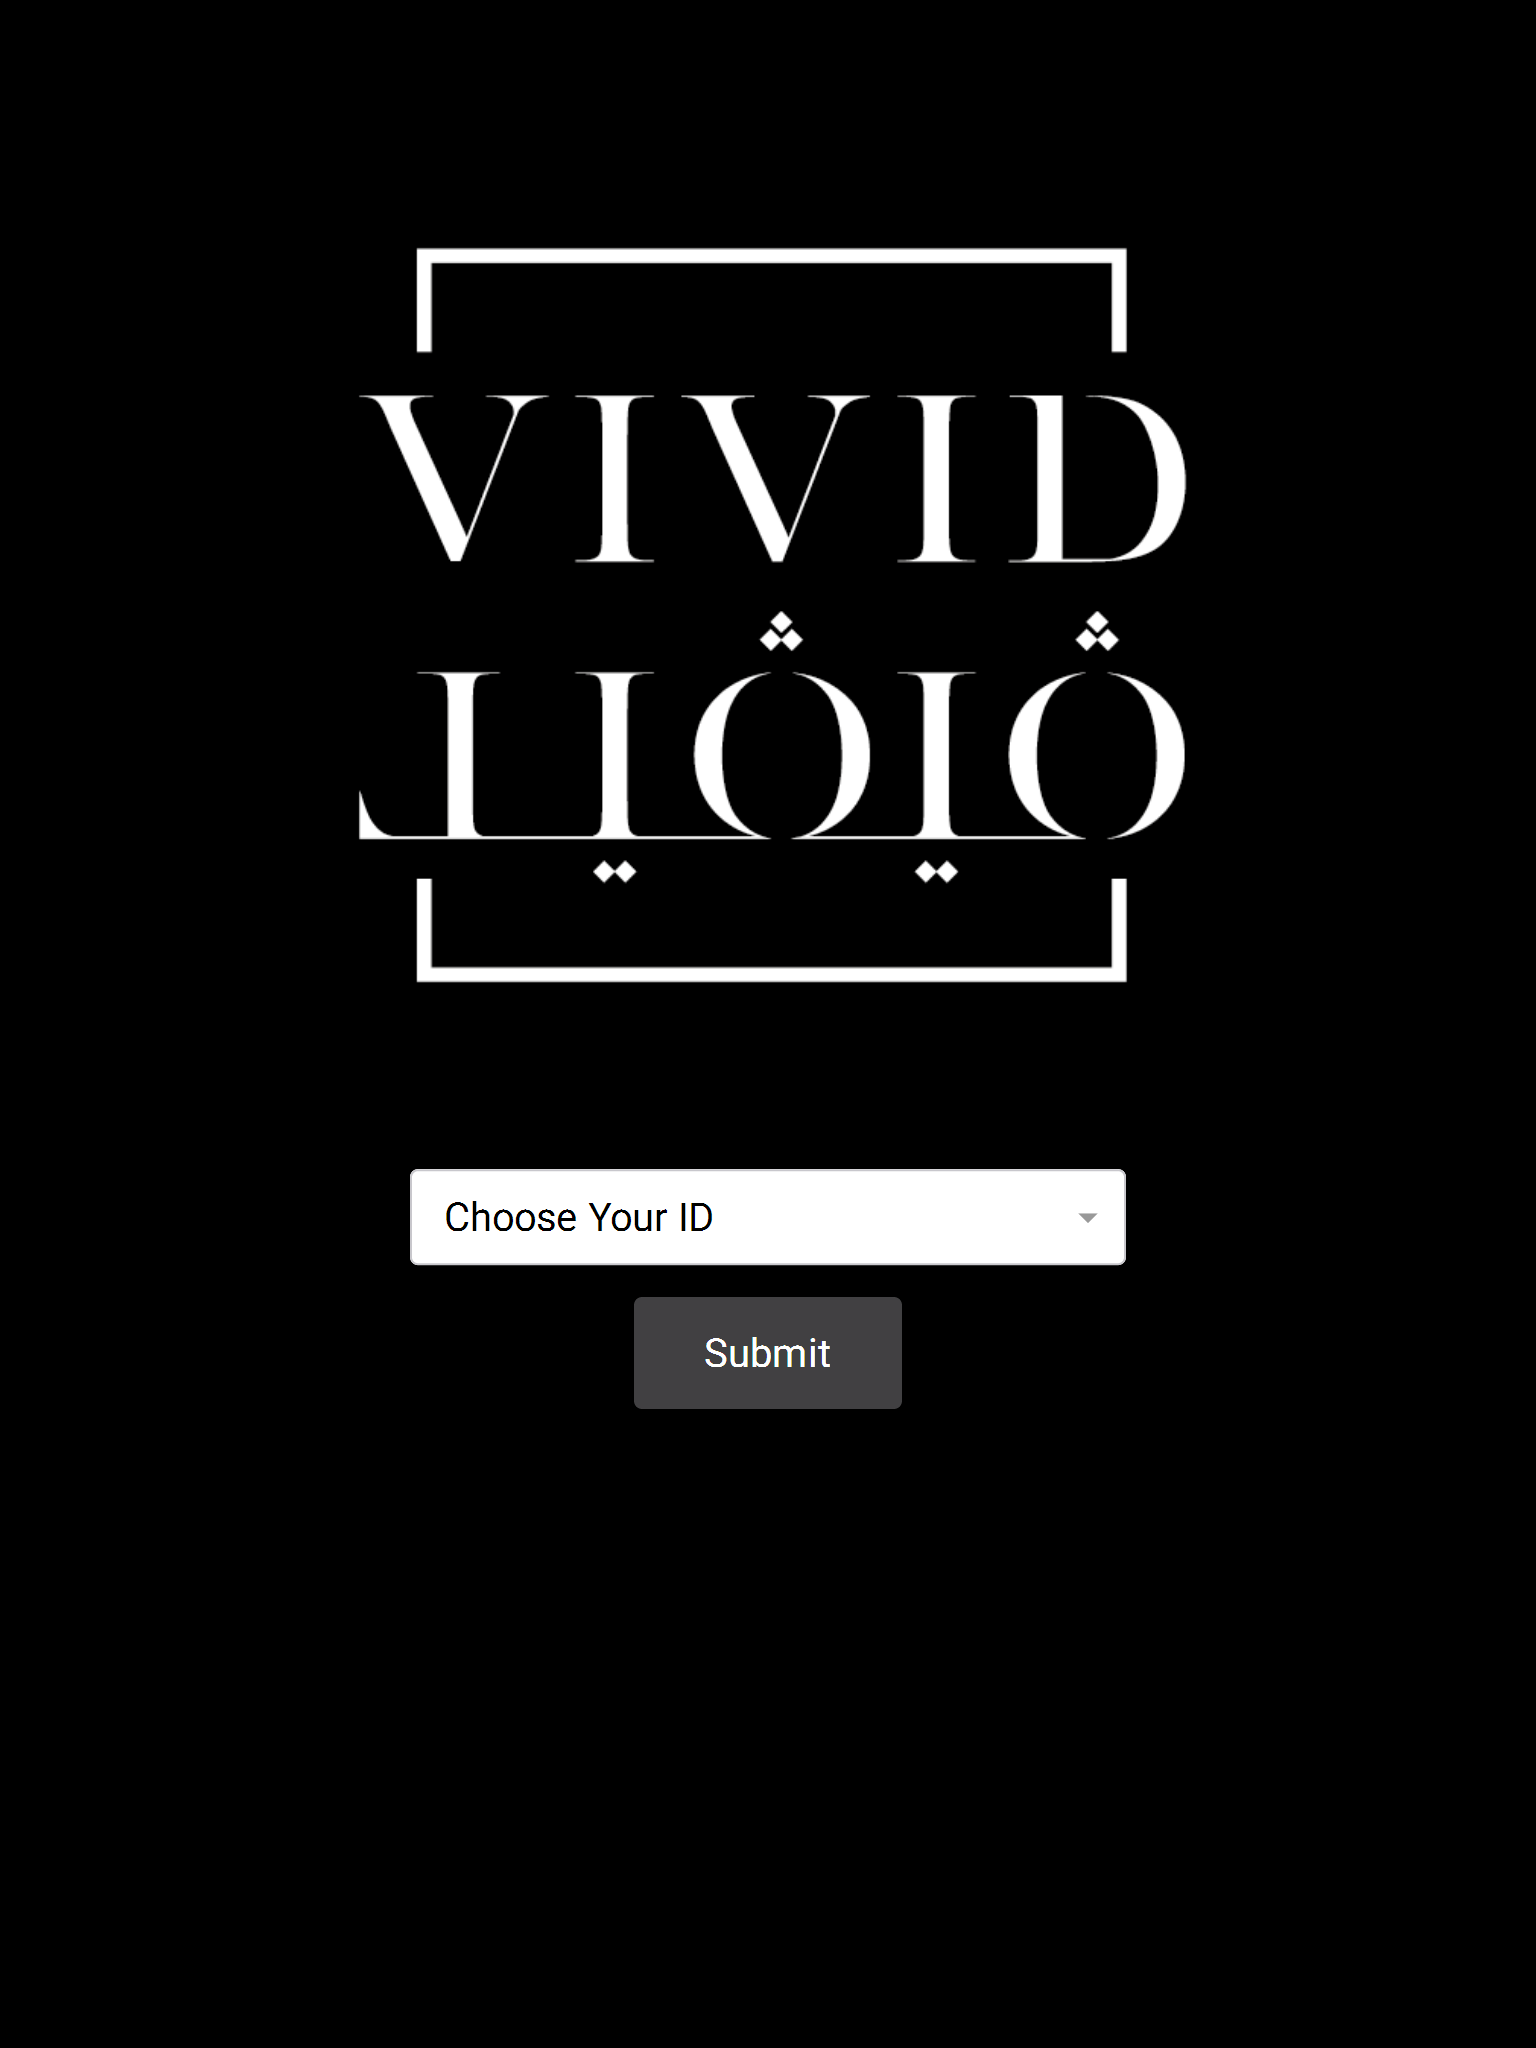
\includegraphics[height=1.1\textwidth]{a.PNG}
\caption{Home Page}
\end{figure}
\newpage
\begin{figure}[h!]
\centering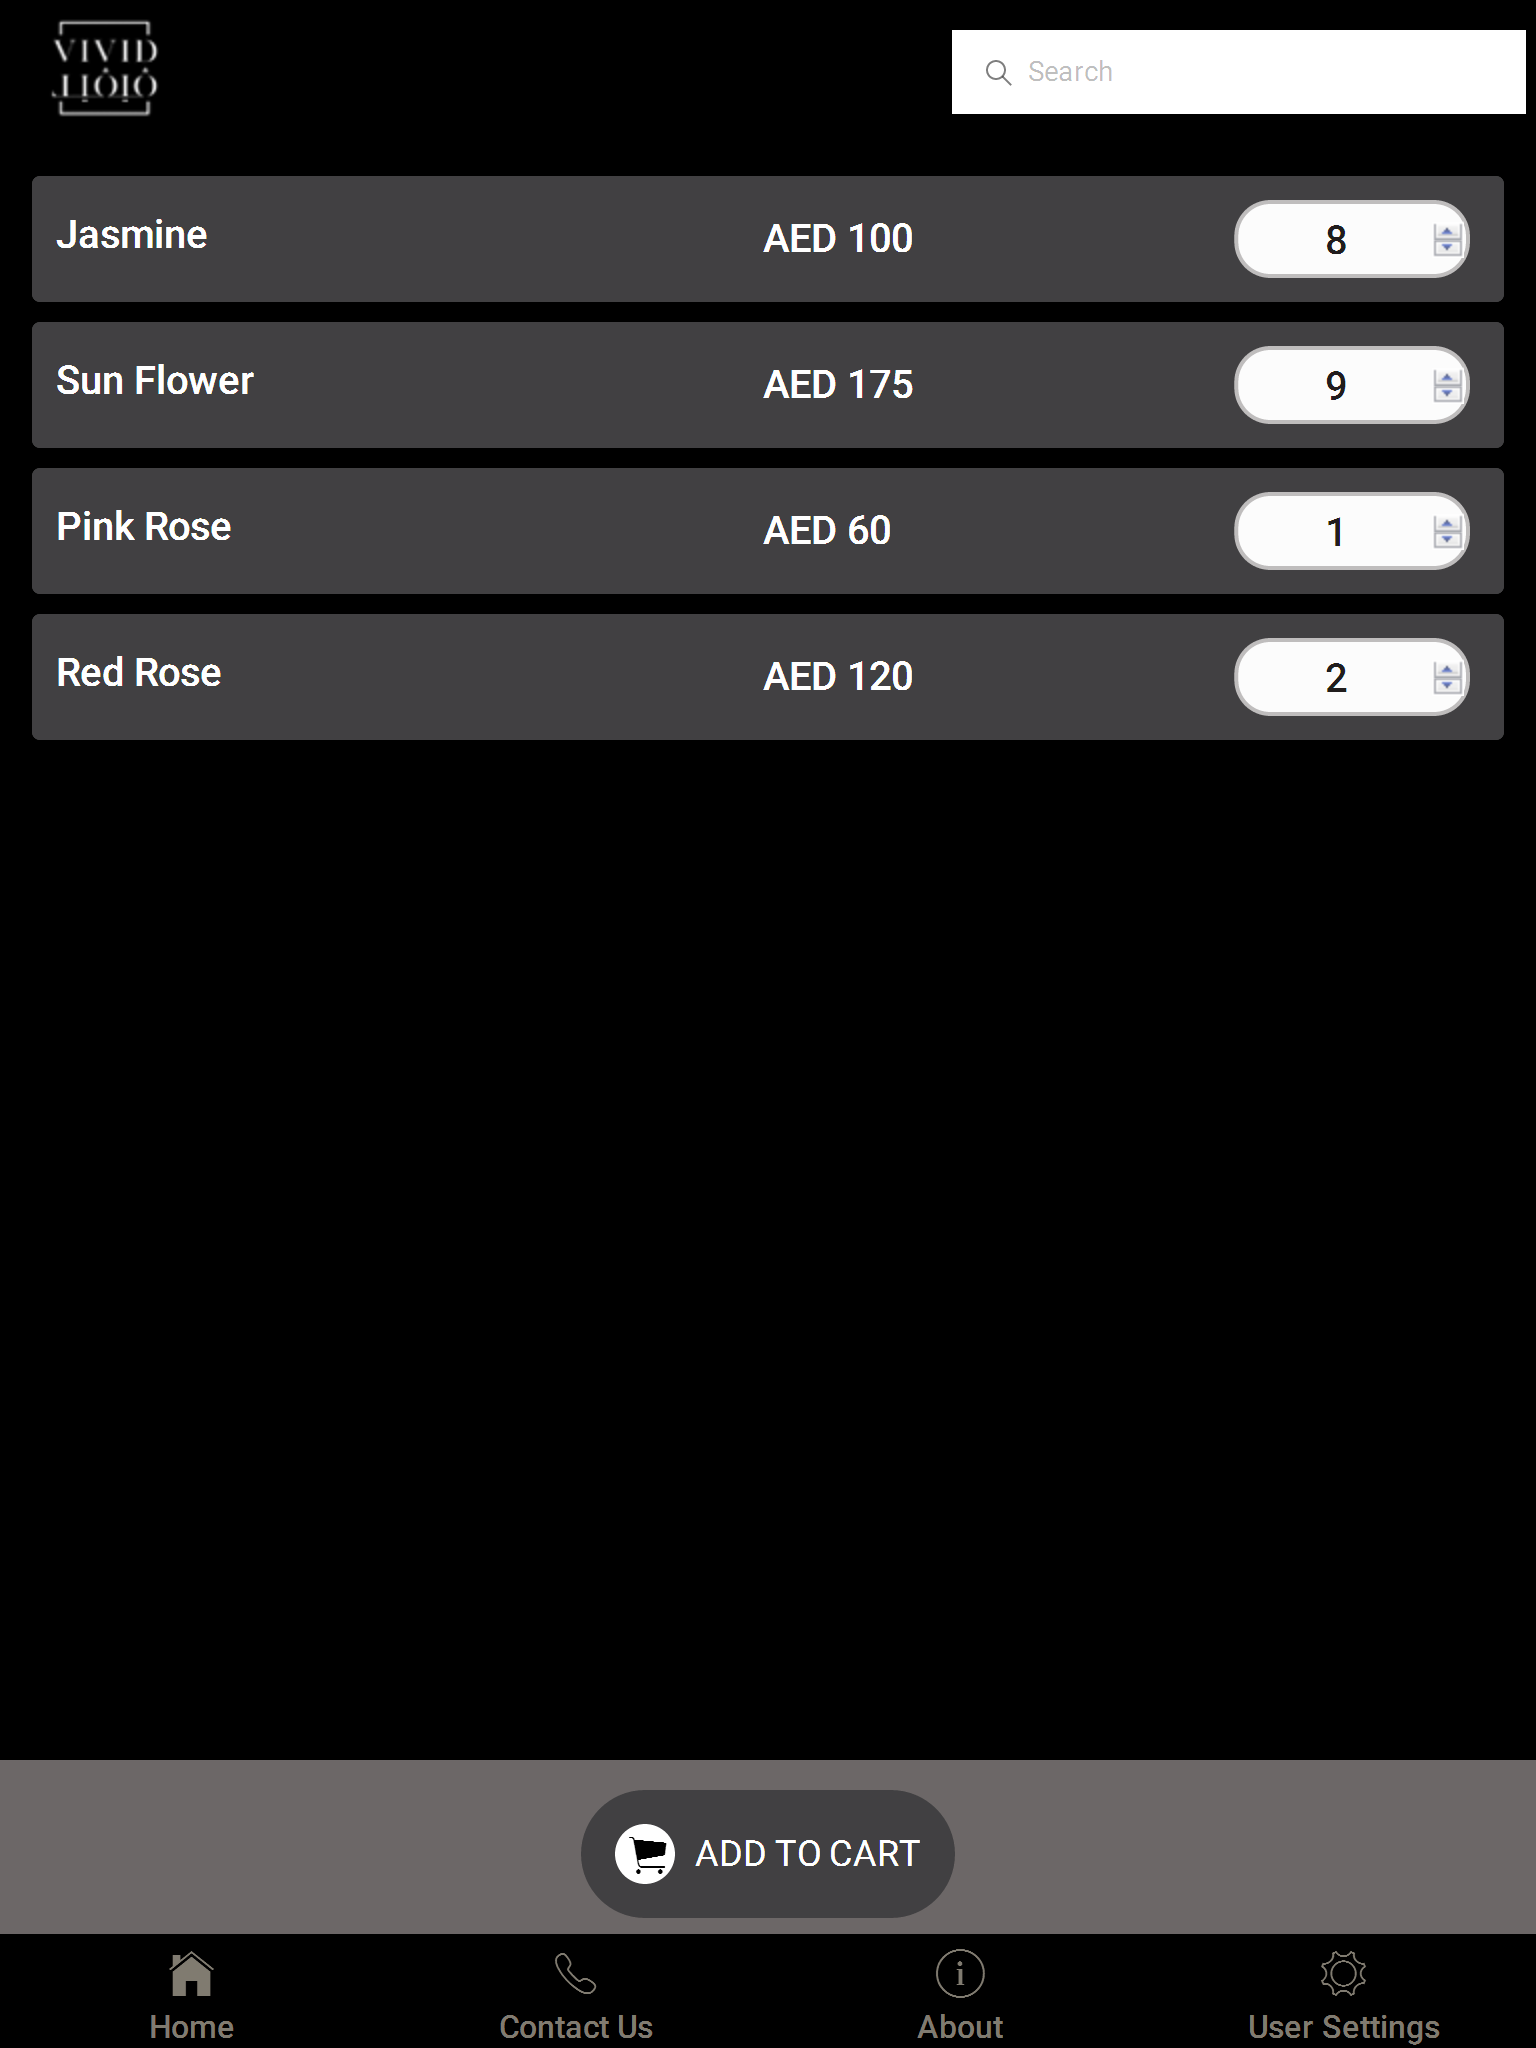
\includegraphics[height=1.1\textwidth]{b.png}
\caption{Stock page}
\end{figure}
\newpage
\begin{figure}[h!]
\centering\includegraphics[height=1.1\textwidth]{c.png}
\caption{Order Page}
\end{figure}
\newpage
\begin{figure}[h!]
\centering
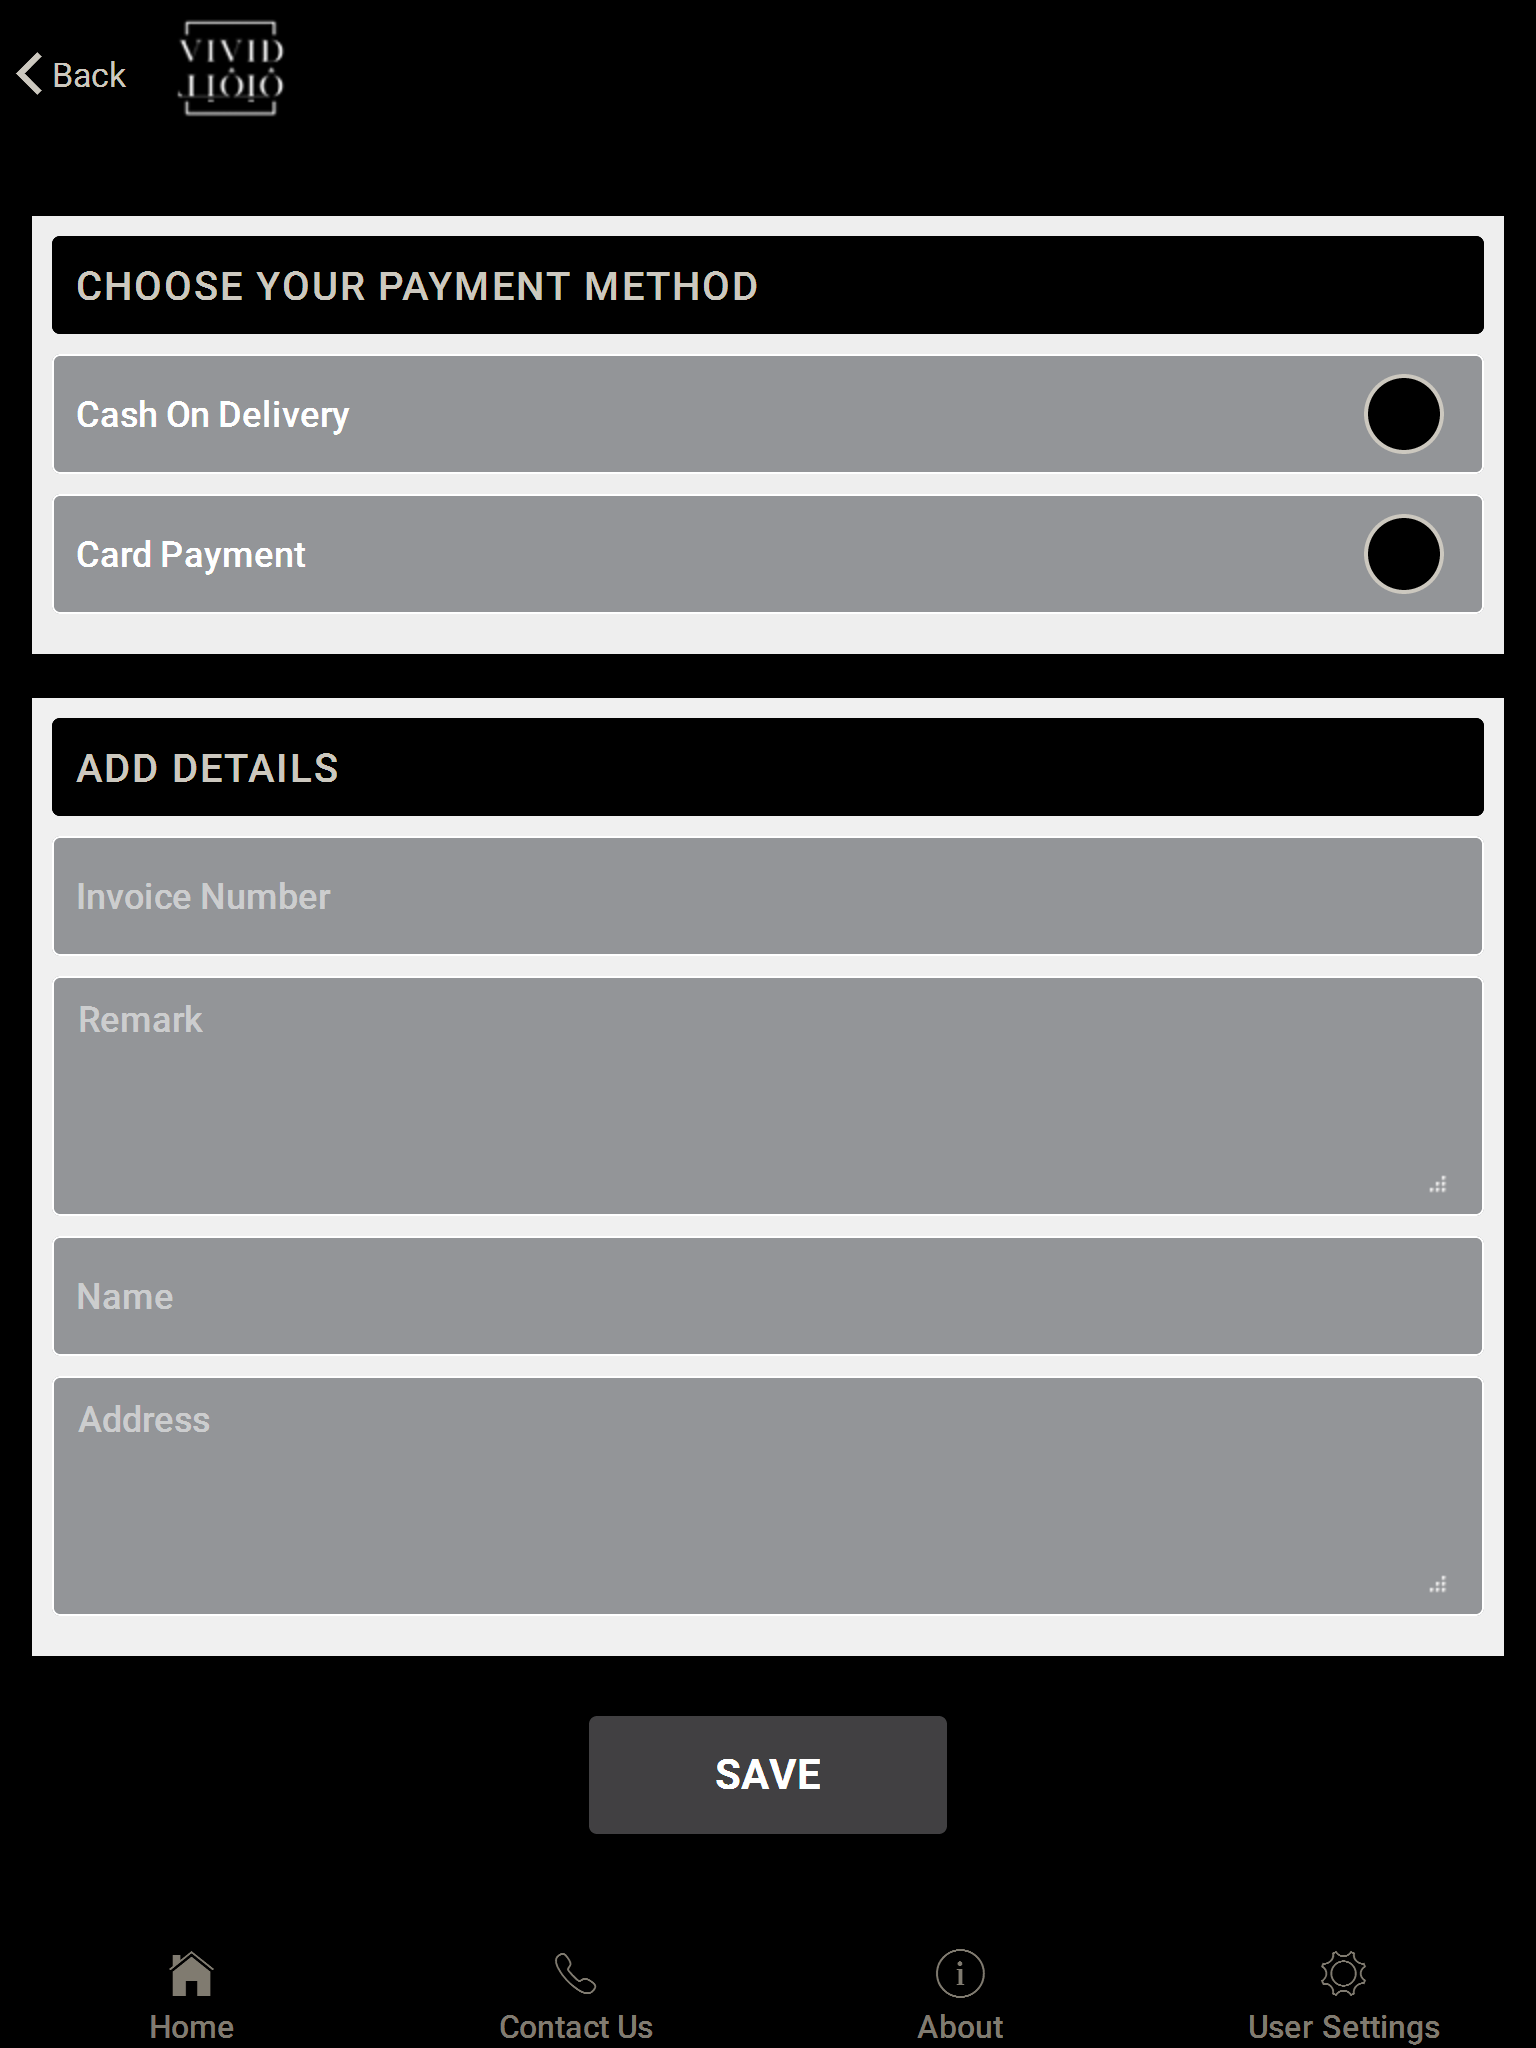
\includegraphics[height=1.1\textwidth]{d.png}
\caption{Payment Page}
\end{figure}
\newpage
\begin{figure}[h!]
\centering
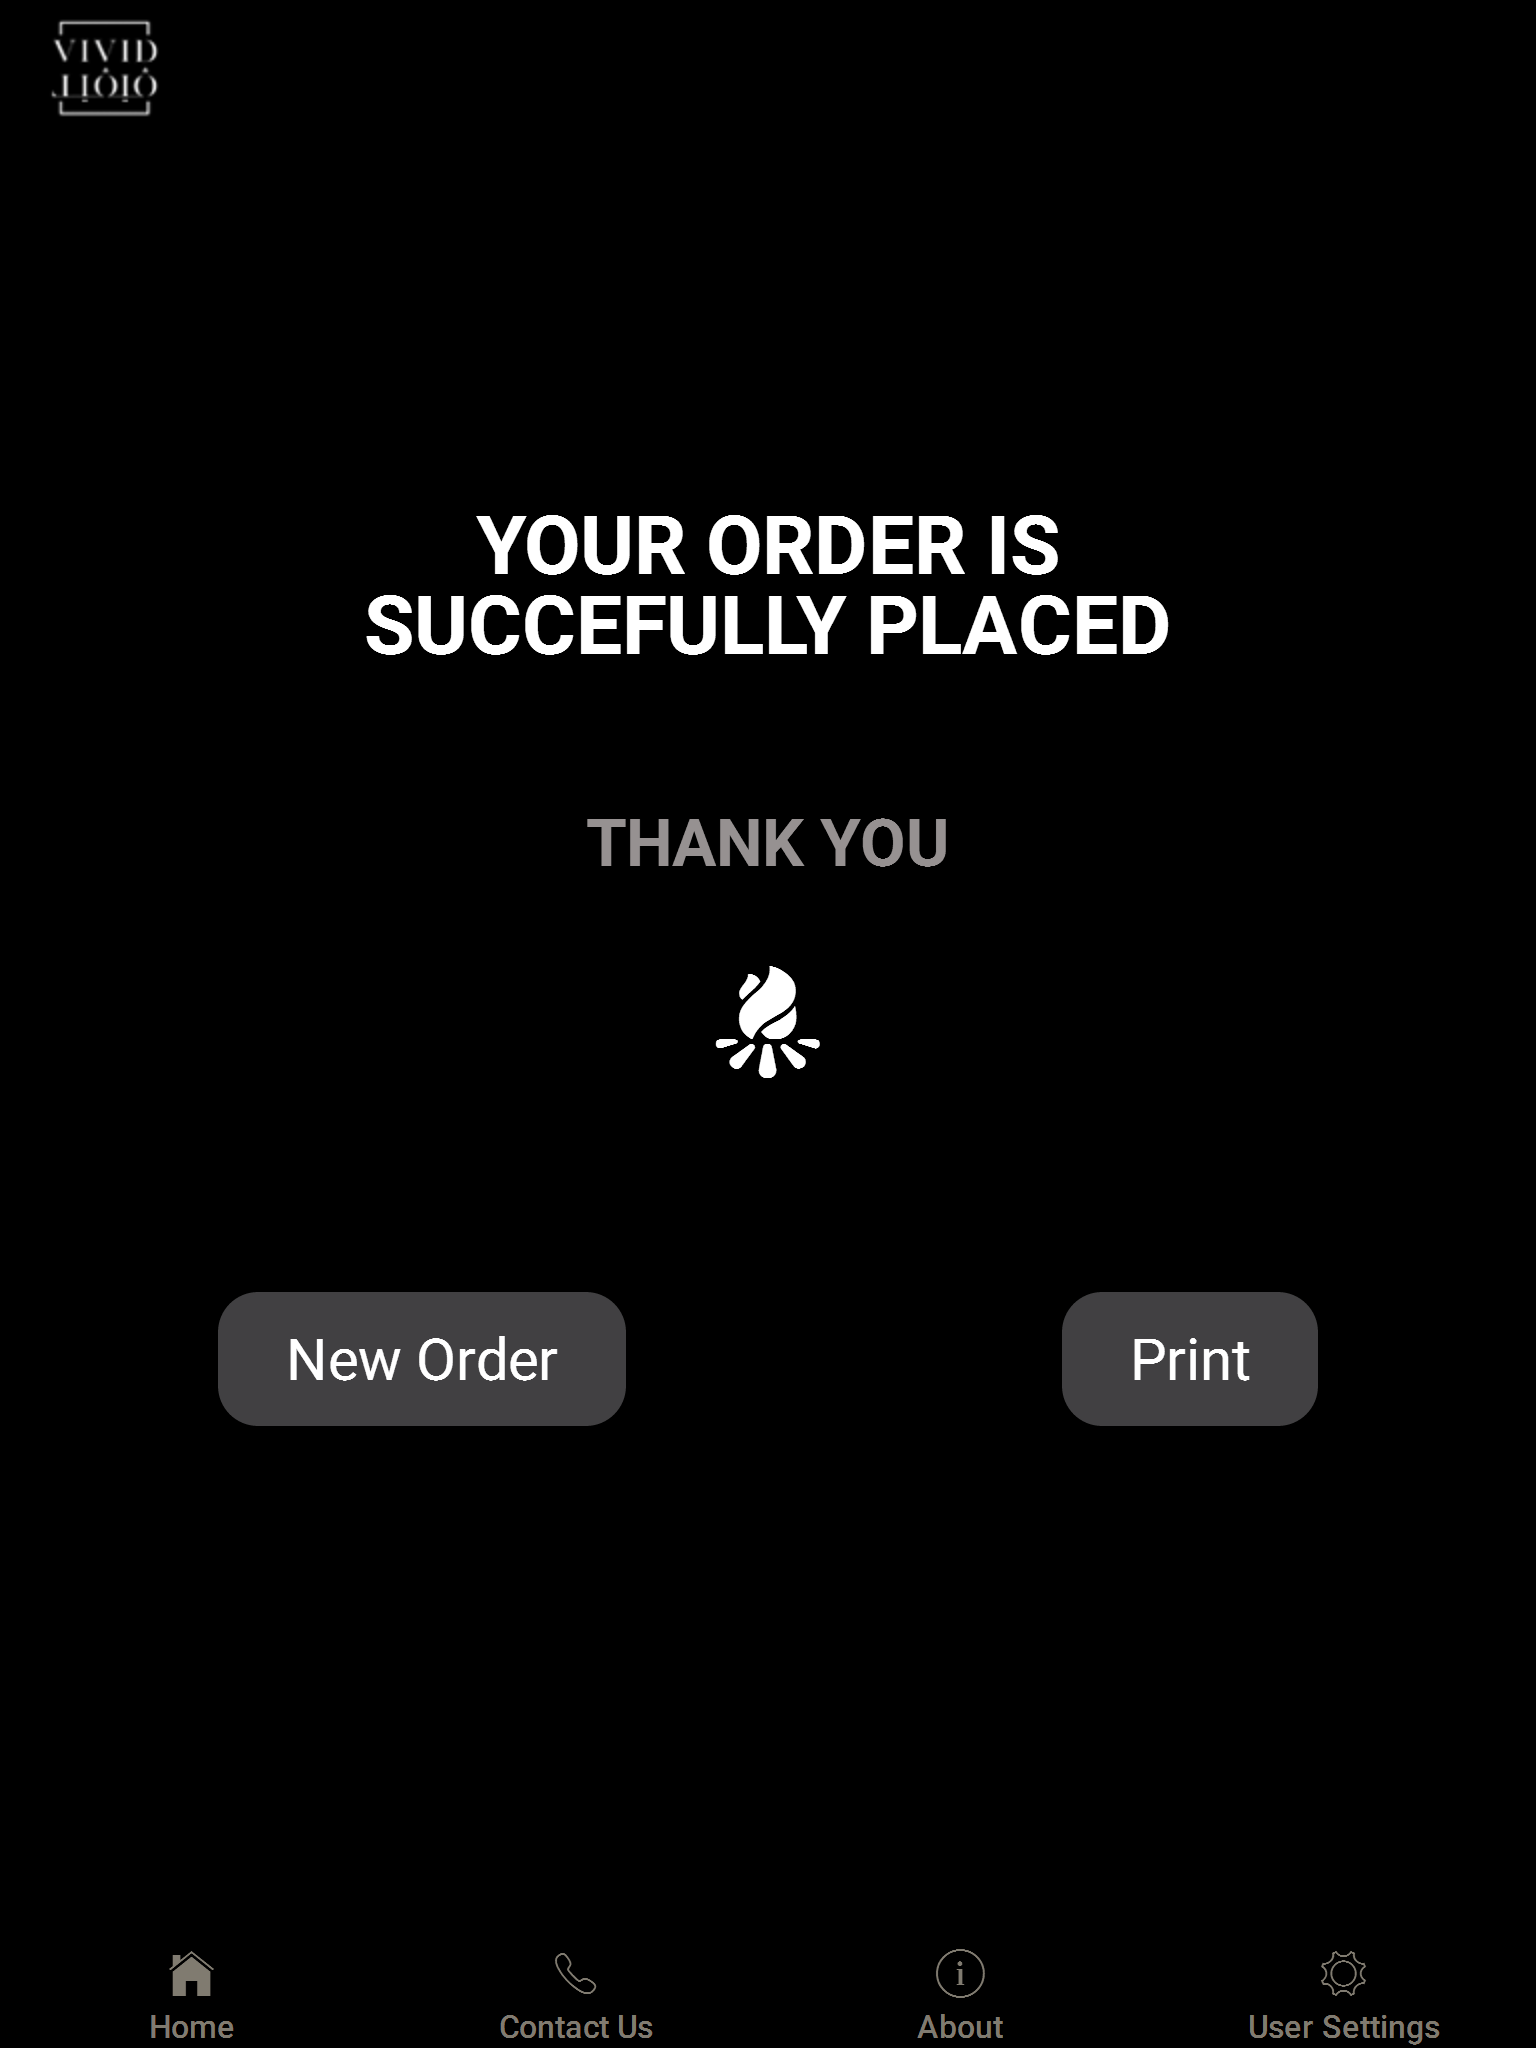
\includegraphics[height=1.1\textwidth]{e.png}
\caption{Thanks Page}
\end{figure}
\newpage
\begin{figure}[h!]
\centering
\includegraphics[height=1.1\textwidth]{f.png}
\caption{Log in page}
\end{figure}
\newpage
\begin{figure}[h!]
\centering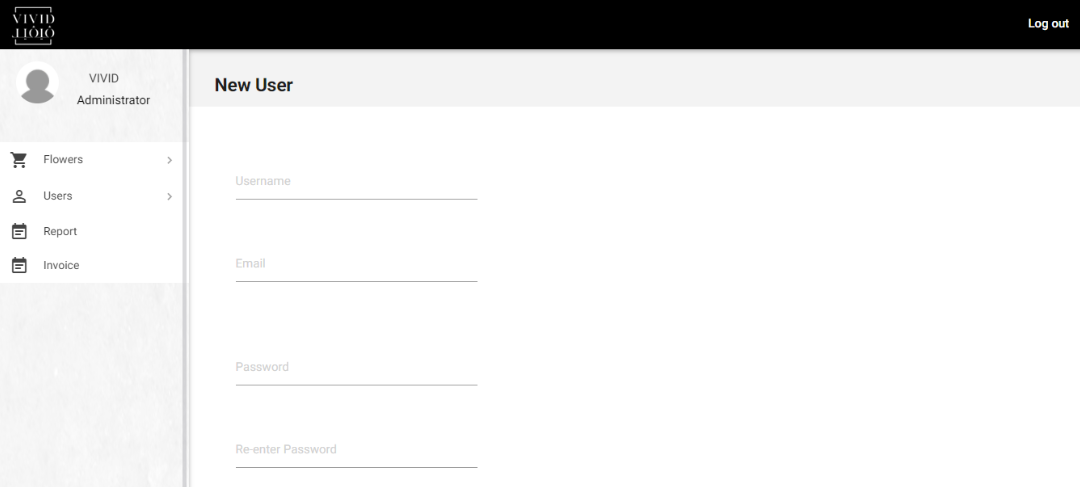
\includegraphics[height=1.1\textwidth]{g.png}
\caption{New user page}
\end{figure}
\newpage
\begin{figure}[h!]
\centering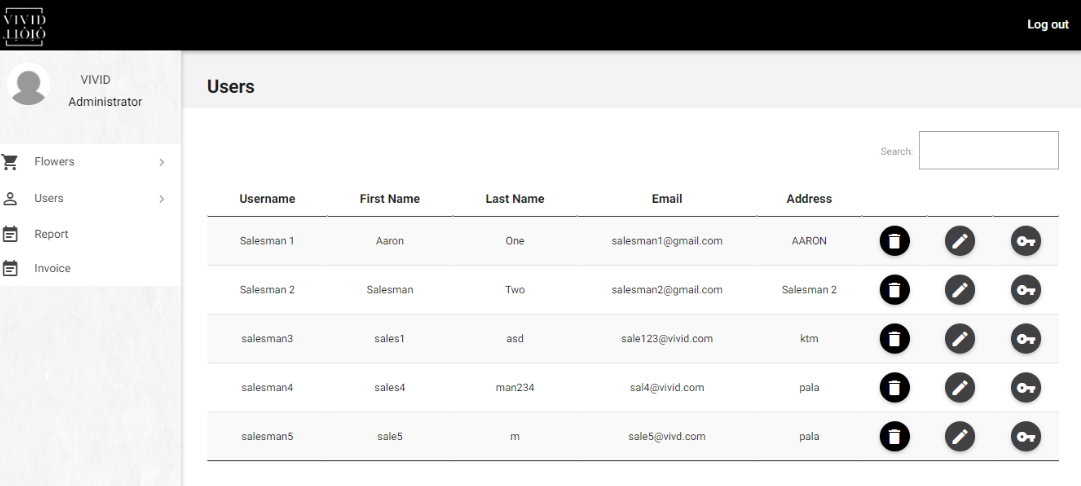
\includegraphics[height=1.1\textwidth]{h.png}
\caption{ User page}
\end{figure}
\newpage
\begin{figure}[h!]
\centering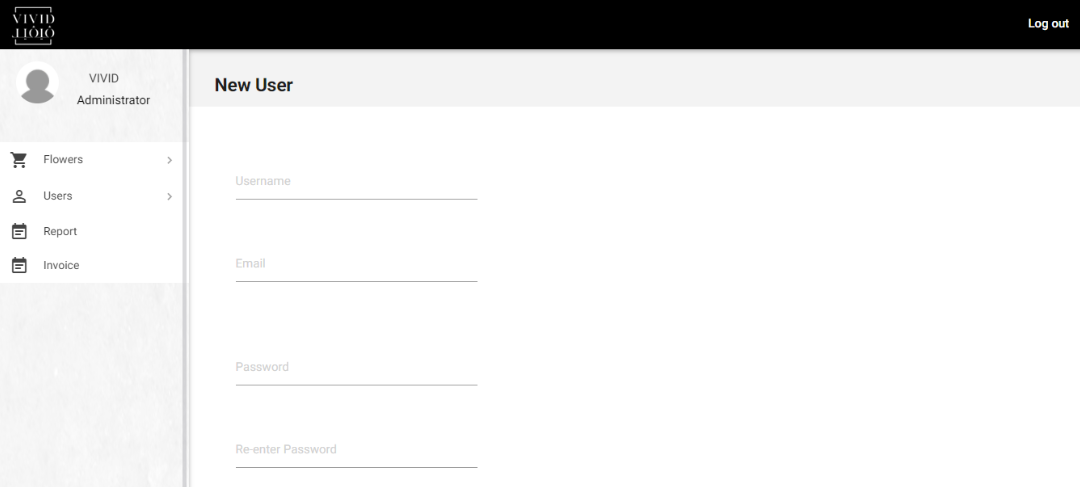
\includegraphics[height=1.1\textwidth]{g.png}
\caption{Flower Stock page}
\end{figure}
\newpage
\begin{figure}[h!]
\centering\includegraphics[height=1.1\textwidth]{k.png}
\caption{Report page}
\end{figure}
\newpage 
\subsection{Appendix C}\vspace{5mm}
\subsubsection{Acronyms}\vspace{5mm}
\begin{enumerate}
\item PHP- Hypertext Preprocessor
\item SEO - Search Engine Optimization
\item SQL - Structured Query Language
\item JVM- Java Virtual Machine
\item SDK - Software Development Kit
\item CSS - Cascading Style Sheet
\item QA - Quality Assurance
\end{enumerate}
\subsubsection{Bibliography}\vspace{5mm}
\begin{thebibliography}{10}
\bibitem{latexGuide} System Analysis and Design   - ELIAS M.AWAD                                                        
\bibitem{latexGuide}Software Engineering   -ROGER.S.PRESSMAN
\bibitem{latexGuide} Visual Basic .NET Black Book-STEVAN HOLZER                                
 \bibitem{latexGuide}\texttt{http://www.google.co.in}.
 \bibitem{latexMath}\texttt{http://www.wikipedia.org}.
 \end{thebibliography}
\end{document}